% !TEX root = presentacion.tex
% Contenido de la presentación del TP6 (medios). Lo usan presentacion.tex y guion.tex.
% Cada diapositiva indica quién expone (\orador) y lo que dice (\note).
% Dos vueltas: Arteaga Barrera, Monja, Mendes Rosa, Baccino, Arteaga Barrera, Monja, Mendes Rosa, Baccino.
% Vuelta 1: medición, AM, FM, televisión analógica y digital (Parte 1).
% Vuelta 2: niveles y ejercicio (Parte 2), DVB-C, DOCSIS, RF Overlay, ISDB-Tb, ISDB-Tb sobre cable (Parte 3) y conclusiones.

% =====================================================
% ---------- Portada ----------
% =====================================================
\begin{frame}[plain]
  \begin{tikzpicture}[remember picture, overlay]
    \node[anchor=east, xshift=1.2cm, yshift=-0.5cm, opacity=0.65] at (current page.east) {
      
\includegraphics[height=0.9\paperheight]{decoracion_a.png}
    };
    \fill[unc verde] (current page.north west) rectangle ([yshift=-1.6cm]current page.north east);
    \node[
      fill=unc verde, text=white, rounded corners=3pt,
      blur shadow={shadow blur steps=5, shadow xshift=0pt, shadow yshift=-3pt, shadow opacity=40},
      inner sep=12pt, minimum width=0.88\paperwidth, align=center, font=\Large\bfseries
    ] at ([yshift=-2.6cm]current page.north) {
      Sistemas de Radiocomunicación \\ Actividad 6: Medios
    };
    \node[anchor=center, text width=0.85\paperwidth, align=center] at ([yshift=-1.4cm]current page.center) {
      {\large\bfseries Mediciones en medios de comunicación analógicos y digitales}\\[0.25cm]
      {\normalsize Arteaga Barrera, Cristian Eduardo\\Baccino, Luca\\ Mendes Rosa, Agustín\\ Monja, Ernesto Joaquín}\\[0.25cm]
      {\small Facultad de Ciencias Exactas, Físicas y Naturales -- Universidad Nacional de Córdoba}\\[0.15cm]
      {\small Córdoba, 2026}
    };
    \node[anchor=south] at ([yshift=0.1cm]current page.south) {
      
\includegraphics[height=1.2cm]{unc_fcefyn_logo.png}
    };
  \end{tikzpicture}
  \orador{Vuelta 1}{Cristian Arteaga Barrera}
  \note{\textbf{Cristian Arteaga Barrera (apertura):} Buenas. Somos Cristian Arteaga Barrera, Luca Baccino, Agustín Mendes Rosa y Joaquín Monja, y vamos a presentar la Actividad 6, sobre medios de comunicación analógicos y digitales.}
\end{frame}

% =====================================================
\section[Introducción]{Introducción}
\orador{Vuelta 1}{Cristian Arteaga Barrera}
\begin{frame}{Organización de la exposición}
  \centering
  \small
  \renewcommand{\arraystretch}{1.3}
  \begin{tabular}{l>{\raggedright\arraybackslash}p{4.2cm}>{\raggedright\arraybackslash}p{4.6cm}}
    \toprule
    \textbf{Expositor} & \textbf{Primera vuelta (Parte 1)} & \textbf{Segunda vuelta (Partes 2 y 3)} \\
    \midrule
    Arteaga Barrera & Objetivos, equipamiento y procedimiento & Niveles, ejercicio de AM, DVB-C y DOCSIS \\
    Monja & Radiodifusión en AM & Video RF Overlay en redes FTTH \\
    Mendes Rosa & Radiodifusión en FM & ISDB-Tb e ISDB-Tb sobre cable \\
    Baccino & Televisión analógica y digital & Conclusiones \\
    \bottomrule
  \end{tabular}
  \note{\textbf{Cristian Arteaga Barrera:} Vamos a exponer en dos vueltas. En la primera recorremos las mediciones: yo presento cómo medimos, Joaquín la AM, Agustín la FM y Luca la televisión analógica y digital. En la segunda vuelta yo sigo con los niveles en decibeles, el ejercicio y las tecnologías de cable DVB-C y DOCSIS; Joaquín presenta el RF Overlay sobre fibra; Agustín la norma ISDB-Tb y su uso sobre cable; y Luca cierra con las conclusiones.}
\end{frame}

\begin{frame}{Objetivos y estructura de la actividad}
  \begin{columns}[T]
    \begin{column}{0.48\textwidth}
      \begin{block}{Objetivos}
        \small
        \begin{itemize}
          \item Identificar y medir señales con el analizador de espectro
          \item Reconocer el espectro de AM, FM y TV analógica y digital
          \item Relacionarlo con la modulación y la canalización
          \item Interpretar niveles en dBm, dBµV y dBc
          \item Describir la distribución por cable y fibra
        \end{itemize}
      \end{block}
    \end{column}
    \begin{column}{0.5\textwidth}
      \small
      \textbf{Parte 1:} mediciones de AM, FM, TV analógica y TDA.\\[0.2cm]
      \textbf{Parte 2:} niveles y ejercicio de AM.\\[0.2cm]
      \textbf{Parte 3:} DVB-C, DOCSIS, RF Overlay, ISDB-Tb e ISDB-Tb sobre cable.\\[0.3cm]
      Cada servicio se identificó con el plan de frecuencias: CABFRA y canalización de ENACOM.
    \end{column}
  \end{columns}
  \note{\textbf{Cristian Arteaga Barrera:} El objetivo de la actividad es usar el analizador de espectro sobre emisiones reales y relacionar lo que vemos con la modulación y con la canalización de cada servicio. Tiene tres partes: las mediciones de radio AM, FM y televisión analógica y digital; la interpretación de los niveles en decibeles con un ejercicio de AM; y una investigación sobre las tecnologías que distribuyen televisión y datos por cable y por fibra. Para identificar cada banda, canal y frecuencia usamos el plan de frecuencias: el Cuadro de Atribución de Bandas, el CABFRA, y la canalización de ENACOM.}
\end{frame}

% =====================================================
\section[Medición]{Medición}
\orador{Vuelta 1}{Cristian Arteaga Barrera}
\begin{frame}{Equipamiento y conexiones}
  \begin{columns}[T]
    \begin{column}{0.62\textwidth}
      \centering
      \resizebox{\textwidth}{!}{%
      \begin{tikzpicture}[font=\small, node distance=0.5cm,
          b/.style={draw, thick, rounded corners=2pt, fill=blue!8, minimum height=0.9cm, text width=1.9cm, align=center},
          f/.style={-{Stealth}, thick}]
        \node[b, fill=orange!12] (ant) {Antena de varillas};
        \node[b, right=of ant] (dc) {Bloqueador de continua};
        \node[b, right=of dc] (sa) {Analizador GSP-827 ($50\,\Omega$)};
        \node[b, fill=green!10, below=0.6cm of sa] (gen) {Generador AFG-2125};
        \draw[f] (ant) -- (dc); \draw[f] (dc) -- (sa); \draw[f, dashed] (gen) -- (sa);
      \end{tikzpicture}}
      \vspace{0.2cm}

      \raggedright\small
      \begin{itemize}
        \item Sólo señales de recepción, nunca un transmisor
        \item Bloqueador de continua obligatorio
        \item Generador conectado directo, con nivel bajo
        \item Fotos de la antena, los equipos y cada pantalla
      \end{itemize}
    \end{column}
    \begin{column}{0.36\textwidth}
      \centering
      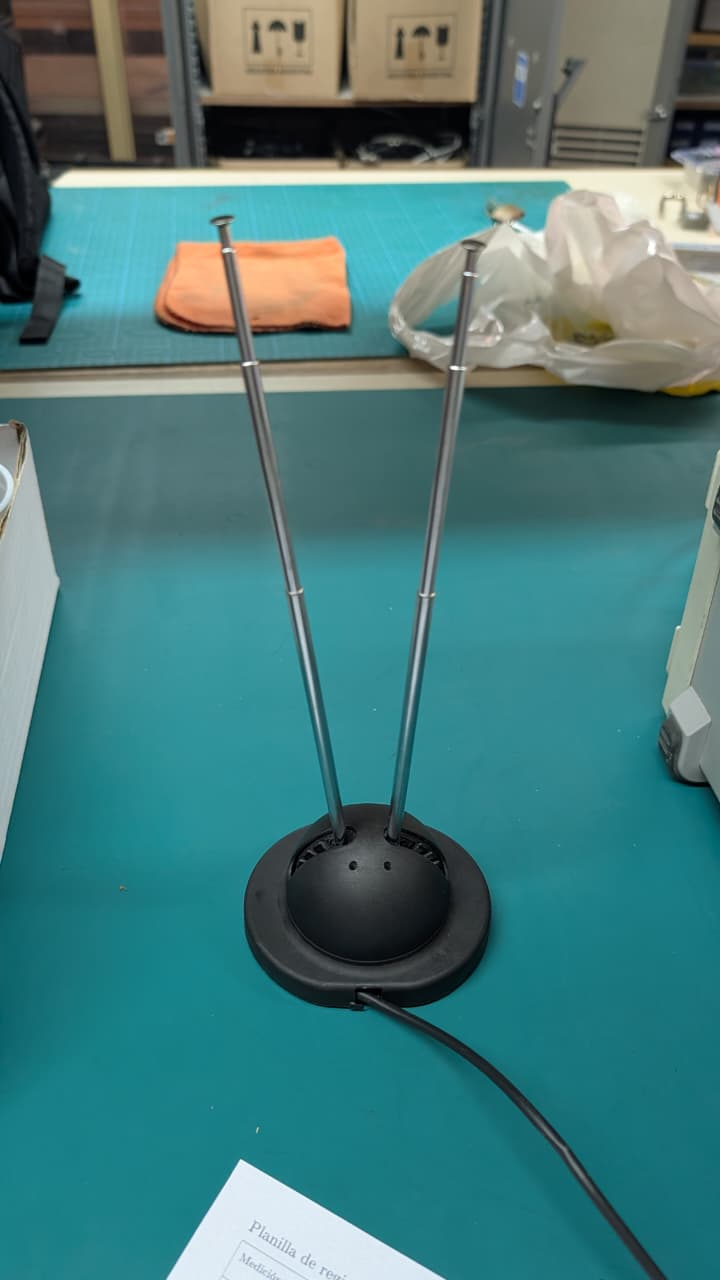
\includegraphics[height=0.66\textheight]{am_antena.png}\\
      {\scriptsize Antena interior de varillas telescópicas}
    \end{column}
  \end{columns}
  \note{\textbf{Cristian Arteaga Barrera:} Medimos con un analizador de espectro GW Instek GSP-827, de 50 ohms. La antena es una antena interior de dos varillas telescópicas, que es un dipolo pensado para VHF. Entre la antena y el analizador va un bloqueador de continua, que la cátedra pide como obligatorio para proteger la entrada. Siguiendo la consigna, medimos sólo señales de recepción, nunca la salida de un transmisor. La única señal conectada directamente fue la de un generador, con nivel bajo, para tener una AM con modulante conocida. De cada medición sacamos foto de la pantalla, y también de la antena y del equipo.}
\end{frame}

\begin{frame}{Configuración registrada en cada medición}
  \begin{columns}[T]
    \begin{column}{0.48\textwidth}
      \begin{block}{Parámetros registrados}
        \small
        \begin{itemize}
          \item Frecuencia central o inicio y fin
          \item \textit{Span}
          \item Nivel de referencia y escala
          \item RBW y VBW
          \item Atenuación y preamplificación
          \item Unidad e impedancia de entrada
        \end{itemize}
      \end{block}
    \end{column}
    \begin{column}{0.5\textwidth}
      \begin{block}{Ajustes de partida (cátedra)}
        \small
        Ref. $-30$ dBm, ganancia 5 a 10 dB, RBW 9 kHz, VBW 100 kHz.
      \end{block}
      \small
      Después se ajustaron a cada señal: RBW de 300 Hz a 9 kHz, ref. de $-20$ a $-98$ dBm. Para los anchos de banda, \textbf{retención de máximos}.
    \end{column}
  \end{columns}
  \note{\textbf{Cristian Arteaga Barrera:} Antes de cada medición registramos la configuración del analizador: frecuencias, span, nivel de referencia, anchos de banda de resolución y de video, atenuación, unidad e impedancia. En el informe cada servicio tiene su tabla con esos datos. Partimos de los ajustes que recomienda la cátedra, pero como pide la consigna, los cambiamos según la señal: por ejemplo, en AM bajamos el RBW a 300 hertz para separar componentes cercanas, y el nivel de referencia fue desde menos 20 dBm con el generador hasta menos 98 en las emisoras más débiles. Como las señales de programa cambian todo el tiempo, para estimar anchos de banda usamos la retención de máximos.}
\end{frame}

\begin{frame}{Impedancias: $50\,\Omega$ y $75\,\Omega$}
  \begin{columns}[T]
    \begin{column}{0.5\textwidth}
      \small
      Analizador: $50\,\Omega$. Antenas y redes de TV: $75\,\Omega$.
      \begin{block}{Conexión directa}
        \[ |\Gamma| = \frac{75 - 50}{75 + 50} = 0{,}2 \]
        \[ L = -10\log\left(1 - |\Gamma|^2\right) \approx 0{,}18 \text{ dB} \]
      \end{block}
    \end{column}
    \begin{column}{0.48\textwidth}
      \small
      \begin{itemize}
        \item La pérdida por desadaptación es despreciable frente a la incertidumbre de lectura
        \item Un adaptador de mínima pérdida atenúa unos 5,7 dB, que hay que sumar a la lectura
        \item La conversión entre dBm y dBµV cambia con la impedancia (Parte 2)
      \end{itemize}
    \end{column}
  \end{columns}
  \note{\textbf{Cristian Arteaga Barrera:} La consigna pide verificar las impedancias. El analizador es de 50 ohms y las antenas y redes de televisión son de 75. Si se conectan directamente, el coeficiente de reflexión es 0,2 y la pérdida por desadaptación es de unos 0,18 dB, que es despreciable frente a lo que podemos leer en la pantalla. Si se usa un adaptador de mínima pérdida, hay que sumarle a la lectura su atenuación, de unos 5,7 dB. Y la impedancia también importa para convertir niveles, como voy a mostrar en la segunda vuelta. Ahora sigue Joaquín con la AM.}
\end{frame}

% =====================================================
\section[AM]{Radiodifusión en AM}
\orador{Vuelta 1}{Joaquín Monja}
\begin{frame}{Modulación AM}
  \begin{block}{Con un tono de frecuencia $f_m$}
    \[
      v_{AM} = E_c\left[1 + m\cos(2\pi f_m t)\right]\cos(2\pi f_c t)
    \]
  \end{block}
  \begin{columns}[T]
    \begin{column}{0.48\textwidth}
      \small
      \begin{itemize}
        \item Portadora fija en $f_c$: no lleva información
        \item Bandas laterales en $f_c \pm f_m$, de amplitud $\frac{m}{2}E_c$: $20\log\frac{m}{2}$ dBc
        \item Ancho de banda: $2 f_{m,max}$
        \item Banda de 535 a 1705 kHz, canales cada 10 kHz
      \end{itemize}
    \end{column}
    \begin{column}{0.5\textwidth}
      \centering
      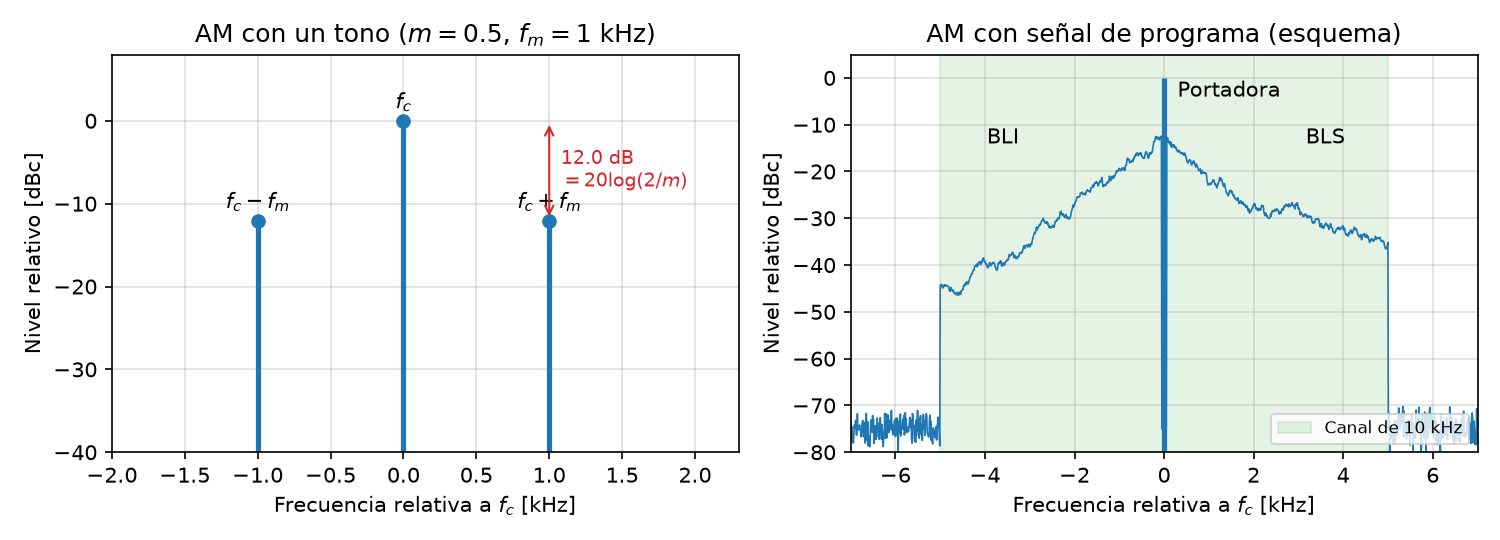
\includegraphics[width=\textwidth]{teoria/am_espectro.png}
    \end{column}
  \end{columns}
  \note{\textbf{Joaquín Monja:} En AM la envolvente de la portadora sigue a la señal modulante. Con un tono, el espectro tiene tres líneas: la portadora, que no depende de la modulación y concentra la mayor parte de la potencia, y dos bandas laterales simétricas, cada una de amplitud m sobre dos por la de la portadora. Con voz o música las bandas laterales se vuelven un espectro continuo que ocupa el doble de la máxima frecuencia modulante. La banda de AM va de 535 a 1705 kHz, con canales separados 10 kHz.}
\end{frame}

\begin{frame}{Exploración de la banda e identificación}
  \begin{columns}[T]
    \begin{column}{0.55\textwidth}
      \centering
      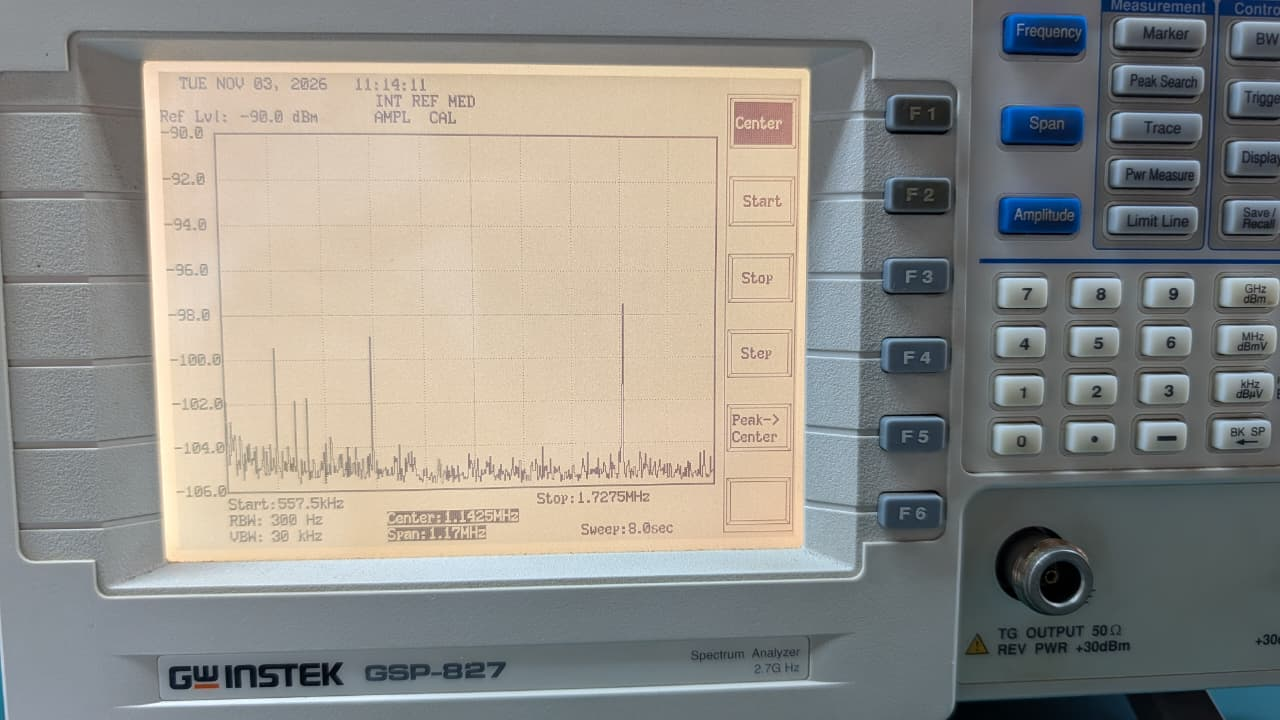
\includegraphics[width=\textwidth]{am_completa.png}\\
      {\scriptsize Banda de AM: 557,5 a 1727,5 kHz, RBW 300 Hz}
    \end{column}
    \begin{column}{0.43\textwidth}
      \small
      \renewcommand{\arraystretch}{1.15}
      \setlength{\tabcolsep}{4pt}
      \begin{tabular}{lll}
        \toprule
        \textbf{Emisora} & \textbf{$f_c$} & \textbf{Nivel} \\
        \midrule
        Cadena 3 & 700 kHz & $-101$ dBm \\
        Radio Mitre & 810 kHz & $-102$ dBm \\
        \bottomrule
      \end{tabular}
      \vspace{0.3cm}

      Identificadas con el plan de frecuencias.\\[0.1cm]
      Piso de ruido: $\approx -104{,}5$ dBm.
    \end{column}
  \end{columns}
  \note{\textbf{Joaquín Monja:} Exploramos la banda de AM y buscamos las señales de mayor nivel. Las dos más fuertes fueron Cadena 3, en 700 kHz, y Radio Mitre, en 810, que identificamos con el plan de frecuencias. Llegaron con unos menos 101 y menos 102 dBm, con el piso de ruido en unos menos 104 y medio. O sea que la portadora quedó apenas 3 dB por encima del ruido, y eso condicionó todo lo que sigue.}
\end{frame}

\begin{frame}{Portadora y bandas laterales}
  \begin{columns}[T]
    \begin{column}{0.49\textwidth}
      \centering
      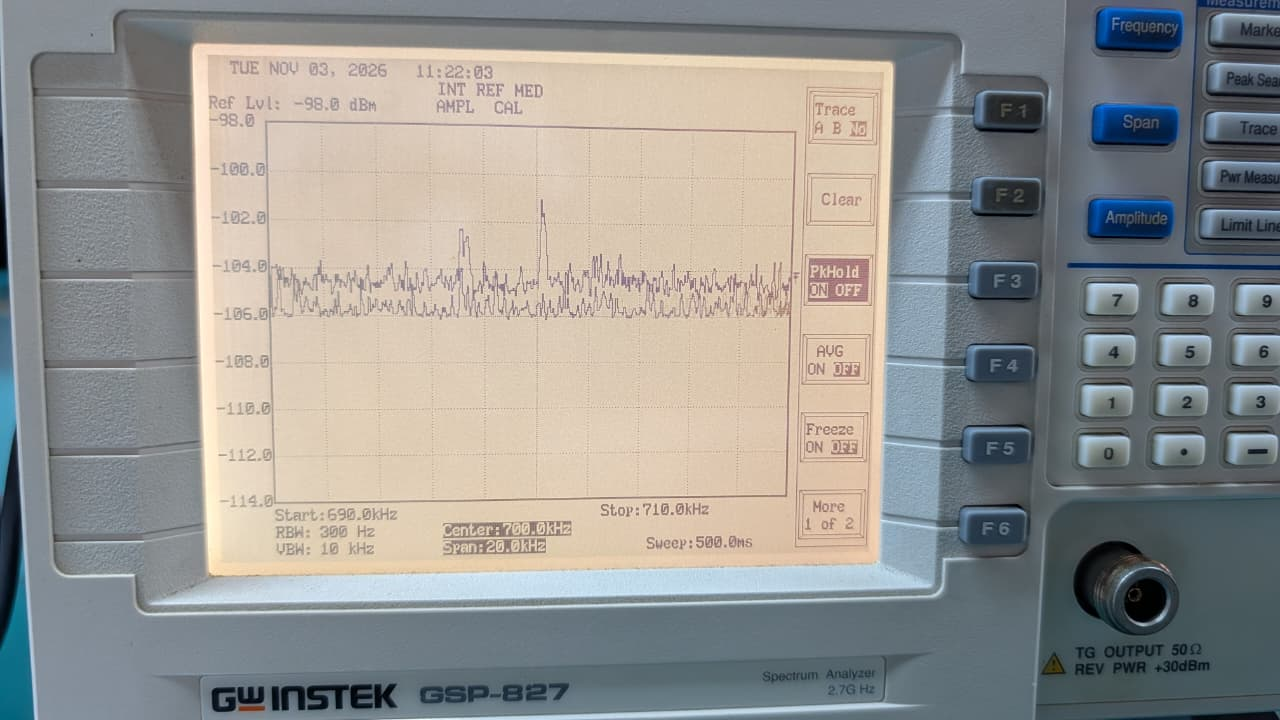
\includegraphics[width=\textwidth]{am_emisora1.png}\\
      {\scriptsize Cadena 3, 700 kHz (\textit{span} 20 kHz)}
    \end{column}
    \begin{column}{0.49\textwidth}
      \centering
      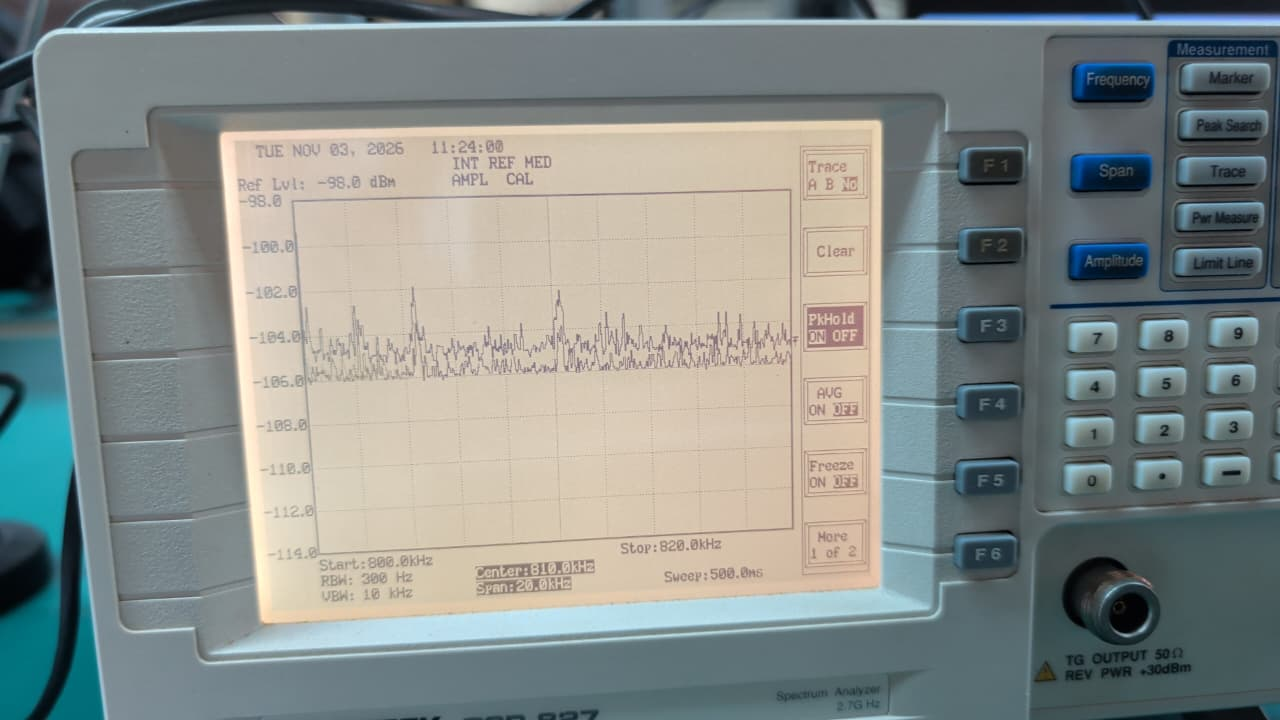
\includegraphics[width=\textwidth]{am_emisora2.png}\\
      {\scriptsize Radio Mitre, 810 kHz (\textit{span} 20 kHz)}
    \end{column}
  \end{columns}
  \vspace{0.15cm}
  \small
  \begin{itemize}
    \item Línea central: la portadora. Las bandas laterales quedan bajo el ruido
    \item Antena: $L \approx 1$ m frente a $\lambda \approx 430$ m $\Rightarrow L/\lambda \approx 0{,}002$
    \item La retención de máximos acumula la envolvente, pero también los picos del ruido
  \end{itemize}
  \note{\textbf{Joaquín Monja:} En el detalle de cada emisora, la línea central es la portadora, en la frecuencia asignada. Las bandas laterales deberían verse a los costados, pero con una señal de programa su potencia se reparte en varios kHz y queda decenas de dB por debajo de la portadora: con sólo 3 dB de margen, quedan bajo el ruido. La causa es la antena: mide alrededor de un metro y en 700 kHz la longitud de onda es de 430 metros, así que casi no entrega potencia. Usamos retención de máximos, que acumula la envolvente, pero también retiene los picos del ruido, así que no mejora la relación señal a ruido.}
\end{frame}

\begin{frame}{Ancho de banda, canales adyacentes y $f_{m,max}$}
  \small
  \begin{block}{Ancho de banda ocupado}
    Criterio previsto: $-26$ dB respecto del máximo (UIT-R SM.328). Requiere que la portadora supere el ruido en más de 26 dB; acá fueron 3 dB $\Rightarrow$ \textbf{no medible}. Según la canalización: $\leq 10$ kHz.
  \end{block}
  \begin{block}{Canales adyacentes}
    En $\pm 10$ kHz (bordes de la pantalla) y $\pm 20$ kHz no hay portadoras. Limitación: no se distingue nada por debajo de $\approx -104$ dBm.
  \end{block}
  \begin{block}{Máxima frecuencia modulante}
    $f_{m,max} = B/2 \approx 5$ kHz (teórico). Válido con doble banda lateral completa, componentes sobre el ruido y observación suficientemente larga.
  \end{block}
  \note{\textbf{Joaquín Monja:} Para el ancho de banda habíamos previsto el criterio de menos 26 dB de la UIT, pero para aplicarlo la portadora tiene que superar el ruido en más de 26 dB, y acá fueron 3. Así que no se pudo medir: según la canalización, con canales cada 10 kHz, la emisión debería ocupar como máximo 10 kHz. En los canales adyacentes, a más o menos 10 y 20 kHz, no vimos otras portadoras, lo que coincide con la planificación, aunque la limitación es que cualquier señal por debajo de menos 104 dBm no se ve. La máxima frecuencia modulante es la mitad del ancho de banda, unos 5 kHz en teoría; medirla exige ver la doble banda lateral completa sobre el ruido durante un tiempo suficiente.}
\end{frame}

\begin{frame}{Señal AM generada: modulante senoidal y cuadrada}
  \begin{columns}[T]
    \begin{column}{0.49\textwidth}
      \centering
      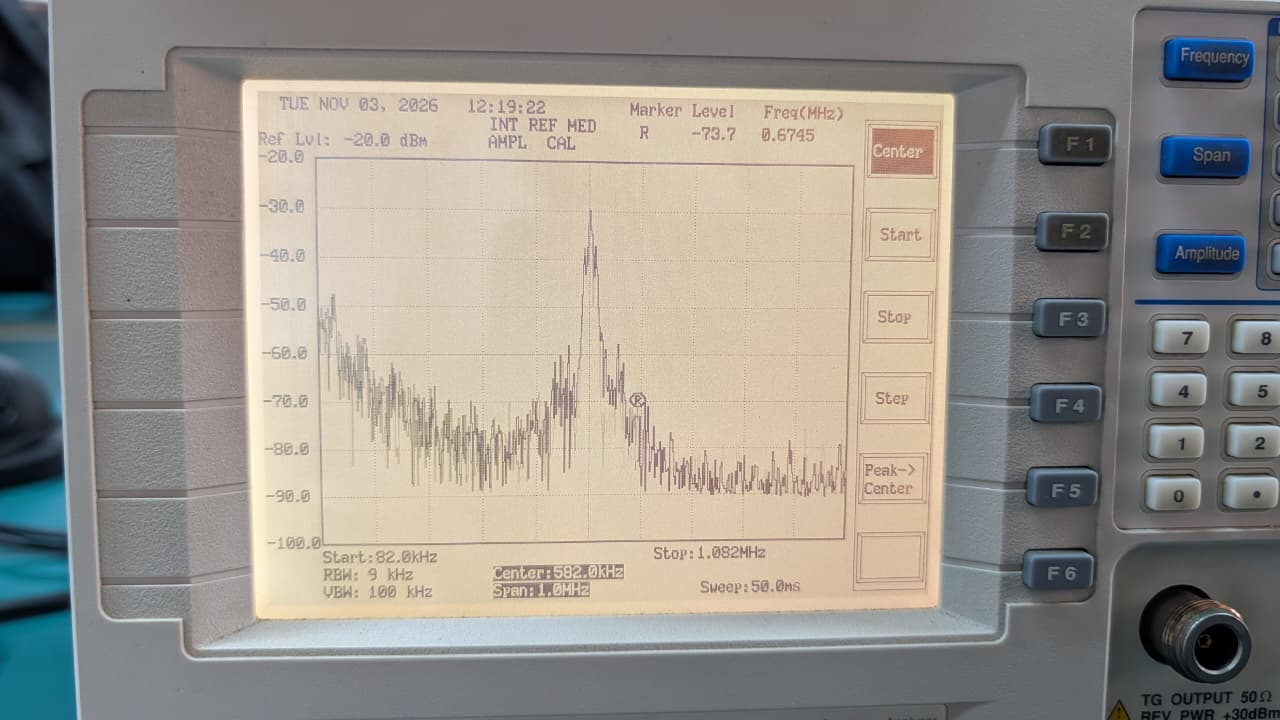
\includegraphics[width=\textwidth]{am_gen_seno.png}\\
      {\scriptsize Senoidal: un solo pico}
    \end{column}
    \begin{column}{0.49\textwidth}
      \centering
      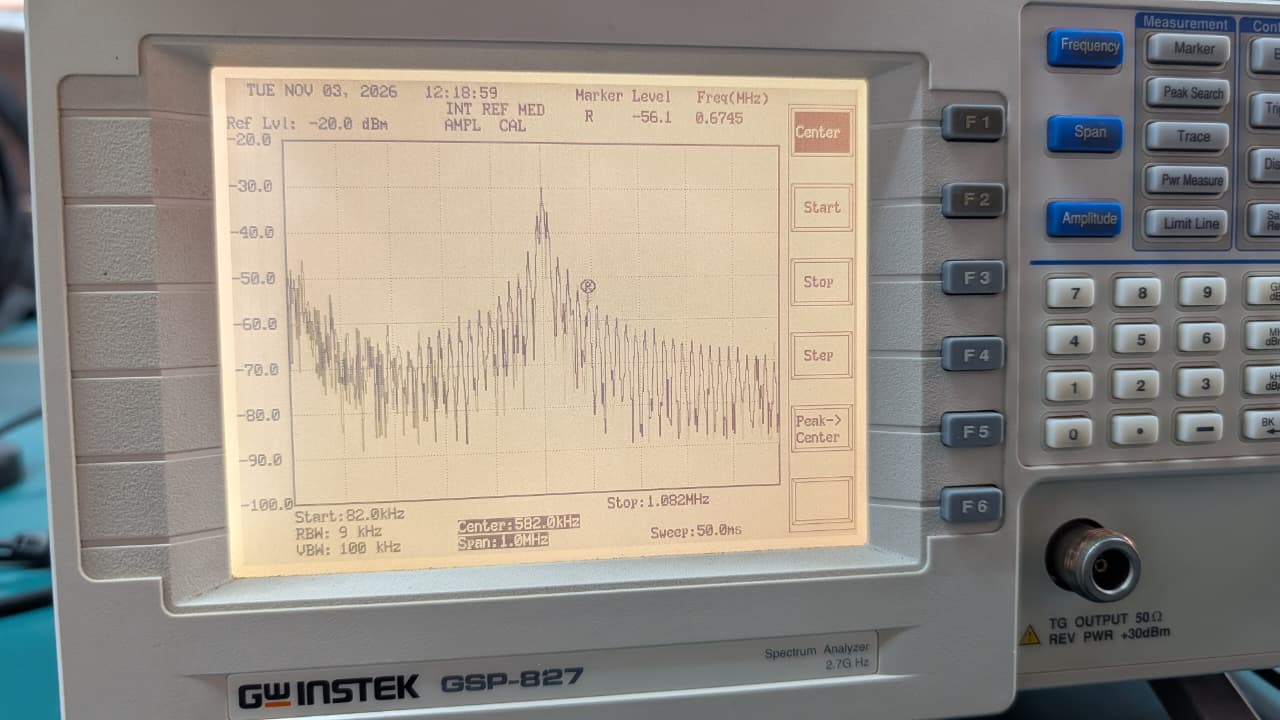
\includegraphics[width=\textwidth]{am_gen_cuadrada.png}\\
      {\scriptsize Cuadrada: peine cada 20 kHz}
    \end{column}
  \end{columns}
  \vspace{0.1cm}
  \small
  AFG-2125: $f_c = 580$ kHz, $-20$ dBm, $f_m = 10$ kHz, $m = 0{,}8$. Analizador: RBW 9 kHz, \textit{span} 1 MHz.
  \begin{itemize}
    \item Senoidal: BL esperadas a $-8$ dBc en $\pm 10$ kHz, no resueltas $\Rightarrow$ $m$ no verificable
    \item Cuadrada: armónicas impares, BL en $f_c \pm n f_m$ con nivel $\propto 1/n$
  \end{itemize}
  \note{\textbf{Joaquín Monja:} Como dice la nota de la consigna, con un generador se puede observar una AM con un tono conocido. Usamos una portadora de 580 kHz, un tono de 10 kHz y una profundidad del 80 por ciento. Con la senoidal, la teoría da dos bandas laterales a menos 8 dBc, pero están a sólo 10 kHz de la portadora y con un RBW de 9 kHz y un span de 1 MHz el analizador no las separa: se ve un solo pico, así que no pudimos medir el índice. Para hacerlo habría que bajar el span a unos 50 kHz y el RBW a 1 kHz. Con la cuadrada aparece un peine cada 20 kHz, porque la cuadrada sólo tiene armónicas impares, de amplitud uno sobre n.}
\end{frame}

\begin{frame}{Índice de modulación y síntesis de AM}
  \begin{block}{Con un único tono}
    \[ m = \frac{2E_{BL}}{E_c} = 2\cdot 10^{(N_{BL} - N_c)/20} \]
  \end{block}
  \small
  \textbf{Con una emisión de programa no se aplica:}
  \begin{itemize}
    \item La modulante tiene muchas componentes variables: no hay una única línea de BL
    \item El nivel depende del RBW y del instante
    \item No puede suponerse $m = 1$: los procesadores limitan los picos
  \end{itemize}
  \textbf{Síntesis:} la información va en la amplitud; portadora fija y BL simétricas de ancho $2f_{m,max}$. El ancho de banda depende del contenido de la modulante: por eso se limita el audio.
  \note{\textbf{Joaquín Monja:} Con un único tono, el índice de modulación sale de la diferencia de nivel entre una banda lateral y la portadora. Con una emisora comercial ese procedimiento no se aplica: la modulante es voz o música, con muchas componentes que cambian todo el tiempo, así que no hay una única línea de banda lateral para medir, y su nivel depende del RBW y del momento. Tampoco se puede suponer que module con m igual a uno: los procesadores de audio limitan los picos para no sobremodular. En síntesis, la AM pone la información en la amplitud, y el espectro es una portadora fija con dos bandas laterales simétricas. Lo que vimos con la cuadrada muestra que el ancho de banda depende de la modulante, y por eso en radiodifusión se limita el audio antes de modular. Sigue Agustín con la FM.}
\end{frame}

% =====================================================
\section[FM]{Radiodifusión en FM}
\orador{Vuelta 1}{Agustín Mendes Rosa}
\begin{frame}{Modulación FM y funciones de Bessel}
  \begin{columns}[T]
    \begin{column}{0.5\textwidth}
      \small
      \[
        v_{FM} = E_c \sum_{n} J_n(\beta)\cos\left[2\pi(f_c + n f_m)t\right]
      \]
      \begin{itemize}
        \item $\beta = \Delta f / f_m$; amplitud constante
        \item Portadora: $E_c J_0(\beta)$; se anula en $\beta = 2{,}405$; $5{,}520$; \dots
        \item Método de la portadora nula: $\Delta f = \beta f_m$
        \item Carson: $B_T \approx 2(\Delta f + f_m)$
      \end{itemize}
    \end{column}
    \begin{column}{0.48\textwidth}
      \centering
      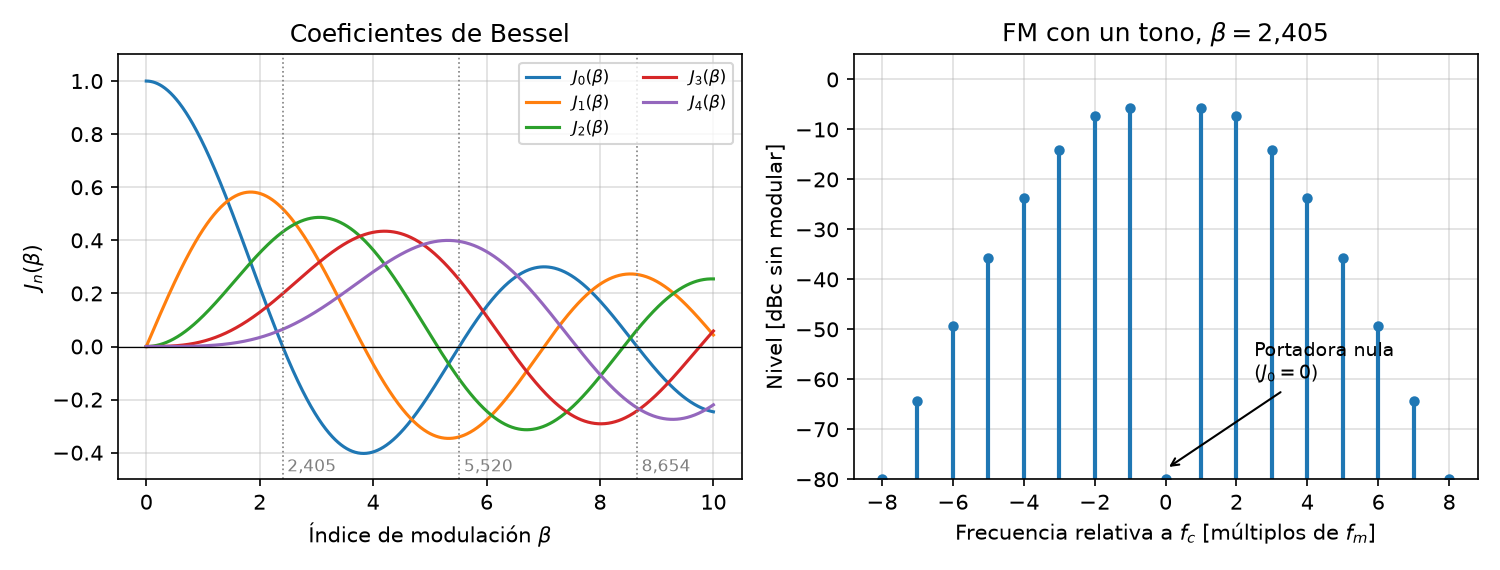
\includegraphics[width=\textwidth]{teoria/fm_bessel.png}
    \end{column}
  \end{columns}
  \note{\textbf{Agustín Mendes Rosa:} En FM lo que cambia es la frecuencia instantánea de la portadora, y la amplitud es constante. Con un tono, el espectro tiene infinitas componentes separadas f m, y la amplitud de cada una es una función de Bessel del índice de modulación beta. La componente en la frecuencia de la portadora vale J cero de beta, que se anula en 2,405 y en otros valores: si con un tono conocido subimos la desviación hasta que la portadora desaparece, obtenemos la desviación con mucha precisión. Ese es el método de la portadora nula de Bessel. Casi toda la potencia queda en el ancho de banda que da la regla de Carson.}
\end{frame}

\begin{frame}{Señal múltiplex estéreo}
  \centering
  \resizebox{0.9\textwidth}{!}{%
    \begin{tikzpicture}[x=0.165cm, y=0.05cm, font=\small]
        \draw[-{Stealth[length=2mm]}] (0,0) -- (80,0) node[right] {$f \, [kHz]$};
        \draw[-{Stealth[length=2mm]}] (0,0) -- (0,108) node[above] {\% de $\Delta f_{max}$};
        \foreach \x in {0,15,19,23,38,53,57,76}
            \draw (\x,0) -- (\x,-1.5) node[below=1pt, font=\scriptsize] {\x};
        \foreach \y in {10,90,100}
            \draw (0,\y) -- (-1,\y) node[left, font=\scriptsize] {\y};
        \draw[densely dotted, gray] (0,100) -- (78,100);
        \draw[thick, blue!70!black, fill=blue!10] (0.03,0) -- (0.03,90) -- (15,90) -- (15,0);
        \node[blue!70!black, align=center] at (7.5,55) {$(L+R)/2$};
        \draw[very thick, red!75!black] (19,0) -- (19,10);
        \node[red!75!black, above] at (19,10) {Piloto};
        \draw[thick, green!45!black, fill=green!10] (23,0) -- (23,90) -- (37.97,90) -- (37.97,0);
        \draw[thick, green!45!black, fill=green!10] (38.03,0) -- (38.03,90) -- (53,90) -- (53,0);
        \node[green!45!black] at (30.5,45) {BLI};
        \node[green!45!black] at (45.5,45) {BLS};
        \node[green!45!black, fill=green!10, inner sep=1pt] at (38,76) {$(L-R)/2$, DBL-PS};
        \draw[dashed, green!45!black] (38,0) -- (38,90);
        \node[green!45!black, font=\scriptsize, fill=white, inner sep=1pt] at (38,22) {38 kHz};
        \draw[thick, orange!80!black, fill=orange!15] (55,0) -- (55,4) -- (59,4) -- (59,0);
        \node[orange!80!black, above] at (57,4) {RDS};
        \draw[decorate, decoration={brace, amplitude=4pt, mirror}] (53,-9) -- (76,-9)
            node[midway, below=5pt, font=\scriptsize, align=center] {Subportadoras adicionales\\($\leq 10$ \%)};
    \end{tikzpicture}}
  \vspace{0.1cm}

  \raggedright\small
  $\Delta f_{max} = 75$ kHz. Receptor estéreo: $L = M + S$, $R = M - S$; mono: sólo $M$. Carson: mono $\approx 180$ kHz, estéreo $\approx 256$ kHz.
  \note{\textbf{Agustín Mendes Rosa:} En radiodifusión la desviación máxima es de 75 kHz, y la portadora no se modula con el audio directamente sino con la señal múltiplex estéreo. Hasta 15 kHz va la suma de los canales, que es lo que usa un receptor mono. En 19 kHz va el tono piloto, que el receptor duplica para regenerar la subportadora de 38 kHz. Alrededor de 38 va la diferencia de canales, en doble banda lateral con portadora suprimida, y en 57 los datos RDS. Con la suma y la diferencia, el receptor estéreo recupera los dos canales. Con Carson, una emisión mono ocupa unos 180 kHz y una estéreo unos 256, frente a canales de 200 kHz.}
\end{frame}

\begin{frame}{Exploración de la banda e identificación}
  \begin{columns}[T]
    \begin{column}{0.55\textwidth}
      \centering
      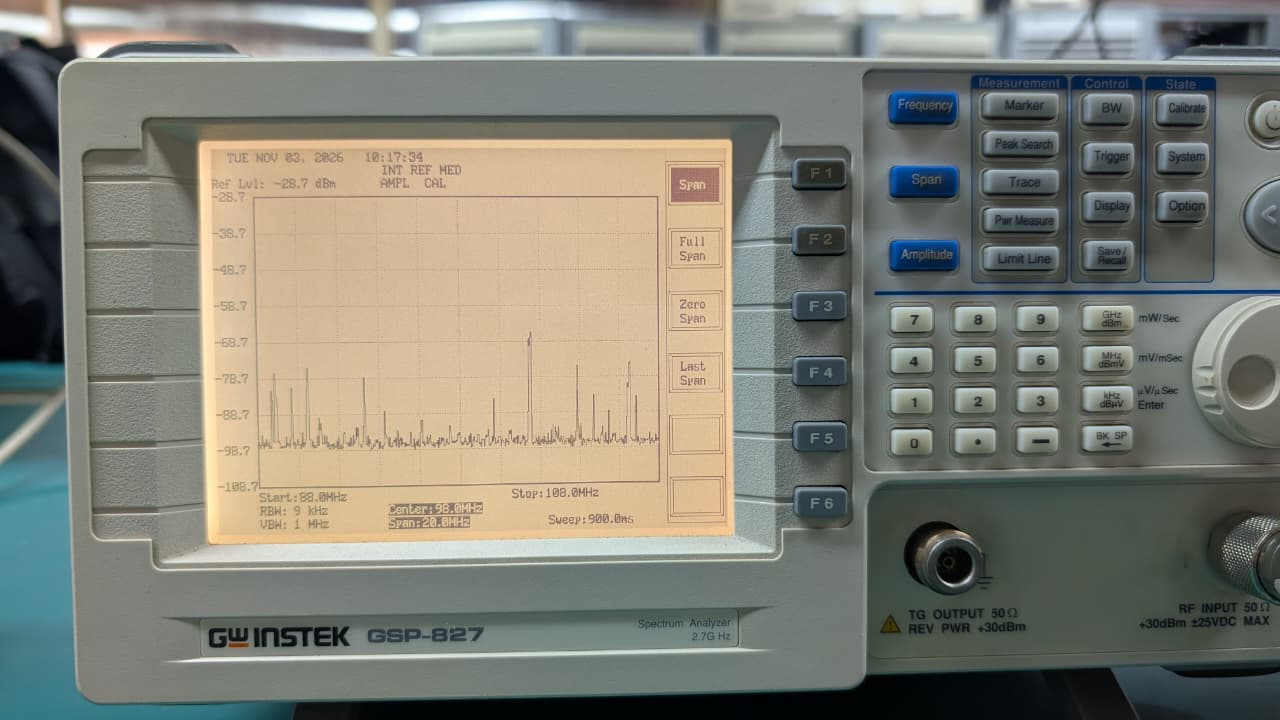
\includegraphics[width=\textwidth]{fm_completa.png}\\
      {\scriptsize Banda de FM: 88 a 108 MHz, RBW 9 kHz}
    \end{column}
    \begin{column}{0.43\textwidth}
      \small
      \begin{itemize}
        \item Una docena de emisoras, de $-90$ a $-65$ dBm
        \item Piso de ruido $\approx -96$ dBm
        \item 88,9 MHz: $\approx -70$ dBm
        \item 102,3 MHz: barrido simple, RBW 300 Hz
      \end{itemize}
      \scriptsize
      No figuran en el listado oficial de ENACOM; según listados no oficiales: Pobre Johnny (88,9) y CBA24 (102,3).
    \end{column}
  \end{columns}
  \note{\textbf{Agustín Mendes Rosa:} En FM la señal llega mucho mejor que en AM, porque la antena es adecuada para VHF. En la banda completa se distinguen alrededor de una docena de emisoras, entre menos 90 y menos 65 dBm. Elegimos dos para el detalle: la de 88,9 MHz, con retención de máximos, y la de 102,3, en un solo barrido con un RBW de 300 hertz. Ninguna de las dos aparece en el listado oficial de ENACOM; según listados no oficiales serían Pobre Johnny y CBA24, las dos de Córdoba.}
\end{frame}

\begin{frame}{Ancho de banda ocupado}
  \begin{columns}[T]
    \begin{column}{0.52\textwidth}
      \centering
      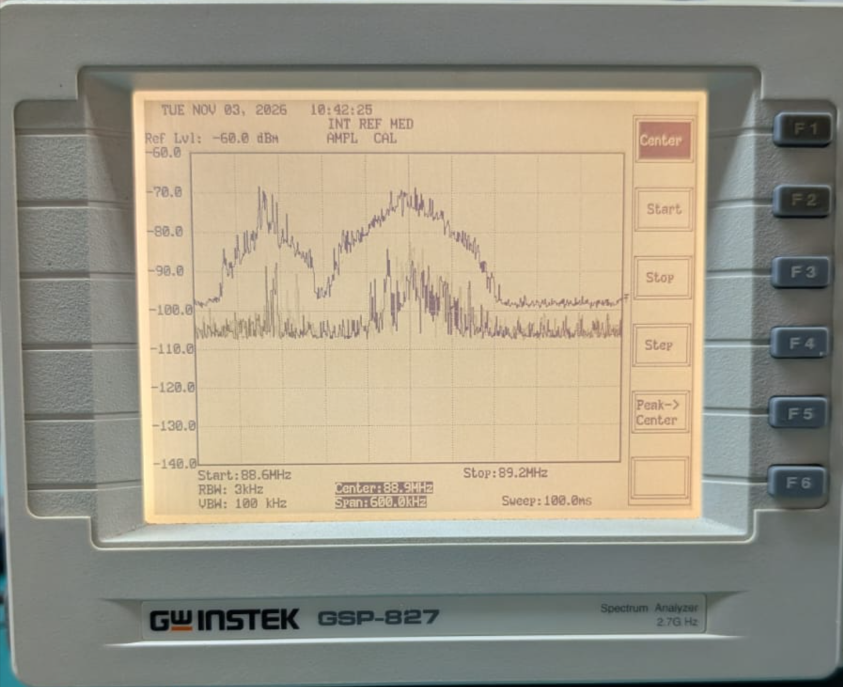
\includegraphics[width=\textwidth]{fm_emisora1.png}\\
      {\scriptsize 88,9 MHz: barrido simple y retención de máximos}
    \end{column}
    \begin{column}{0.46\textwidth}
      \small
      \begin{block}{Criterio: $-26$ dB (UIT-R SM.328)}
        Máximo $\approx -70$ dBm $\Rightarrow$ corte en $\approx -96$ dBm\\
        $B \approx 220$ kHz
      \end{block}
      \begin{itemize}
        \item Canal de 200 kHz: los flancos invaden levemente los vecinos
        \item Entre Carson mono (180) y estéreo (256): estéreo que no siempre alcanza $\Delta f_{max}$
      \end{itemize}
    \end{column}
  \end{columns}
  \note{\textbf{Agustín Mendes Rosa:} Con un programa, la FM no muestra líneas separadas sino un bloque de energía de ancho variable, así que medimos el ancho de banda sobre la envolvente en retención de máximos, con el criterio de menos 26 dB de la UIT. Con el máximo en menos 70, el corte queda en menos 96 dBm, y da unos 220 kHz. Es algo más que el canal de 200 kHz, así que los flancos invaden un poco los canales vecinos, con un nivel muy inferior al del centro. Y queda entre los valores de Carson para mono y estéreo, que es lo esperable para una emisión estéreo que no está siempre en la desviación máxima.}
\end{frame}

\begin{frame}{Canales adyacentes y espectro instantáneo}
  \begin{columns}[T]
    \begin{column}{0.49\textwidth}
      \small
      \begin{block}{Canal adyacente: 88,7 MHz}
        Niveles similares ($\approx -70$ dBm). Los flancos se encuentran en $\approx -98$ dBm, cerca del piso. Bloque más angosto ($\approx 150$ kHz).
      \end{block}
      \textbf{¿Superposición?} La observación no alcanza para confirmarla: el espectro varía, la retención acumula ruido y el efecto depende de la selectividad y del umbral de captura del receptor.
    \end{column}
    \begin{column}{0.49\textwidth}
      \centering
      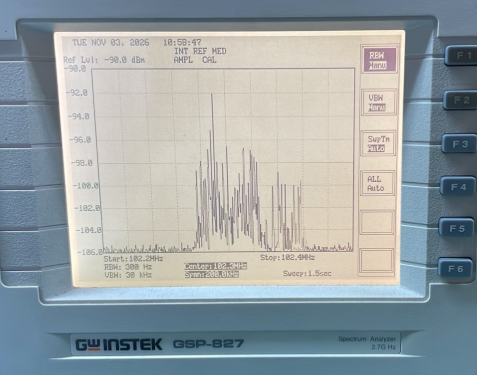
\includegraphics[width=\textwidth]{fm_emisora2.png}\\
      {\scriptsize 102,3 MHz: un solo barrido, RBW 300 Hz}
    \end{column}
  \end{columns}
  \note{\textbf{Agustín Mendes Rosa:} Junto a la emisora de 88,9 apareció otra en 88,7, el canal adyacente, con un nivel parecido. Sus flancos se acercan hasta encontrarse cerca del piso de ruido. Pero la observación no alcanza para afirmar que hay una superposición que interfiera: el espectro cambia con el programa, la retención de máximos también acumula ruido, y el efecto real depende de la selectividad y del umbral de captura del receptor. A la derecha está la de 102,3, en un solo barrido: se ven líneas sueltas, que son las frecuencias donde había energía cuando pasó el filtro. Es el espectro de un instante, y muestra por qué para medir el ancho de banda hay que acumular muchos barridos.}
\end{frame}

\begin{frame}{Índice de modulación con programa y síntesis de FM}
  \small
  \textbf{La relación con $J_0$ no sirve para una emisión de programa:}
  \begin{itemize}
    \item $\beta = \Delta f / f_m$ sólo está definido para un tono; con varios tonos aparecen productos $J_n(\beta_1)J_k(\beta_2)\cdots$
    \item El espectro cambia con el programa: la línea de la portadora sube y baja
    \item La múltiplex incluye piloto, $S$ alrededor de 38 kHz y RDS
  \end{itemize}
  Sobre una emisión real se mide la desviación máxima y se verifica que no supere 75 kHz.
  \vspace{0.2cm}
  \begin{block}{Síntesis}
    Información en la frecuencia instantánea, amplitud constante: robusta frente al ruido, pero ocupa unos 200 kHz frente a 10 kHz de la AM. En el analizador: un bloque de ancho variable con potencia total constante.
  \end{block}
  \note{\textbf{Agustín Mendes Rosa:} La relación con J cero no permite medir el índice de una emisión comercial, por tres razones. El índice beta sólo está definido para un tono, y con varios tonos aparecen productos de intermodulación entre las funciones de Bessel. El espectro cambia todo el tiempo con el programa, así que la línea de la portadora sube y baja. Y además la múltiplex trae el piloto, la diferencia de canales y el RDS. Lo que sí se mide en una emisora real es la desviación máxima, que no debe superar 75 kHz. En síntesis, la FM pone la información en la frecuencia y mantiene la amplitud constante, lo que la hace robusta frente al ruido, a cambio de un ancho de banda veinte veces mayor que el de la AM. Le paso a Luca.}
\end{frame}

% =====================================================
\section[TV analógica]{Televisión analógica}
\orador{Vuelta 1}{Luca Baccino}
\begin{frame}{Canal PAL-N y canalización}
  \begin{columns}[T]
    \begin{column}{0.58\textwidth}
      \centering
      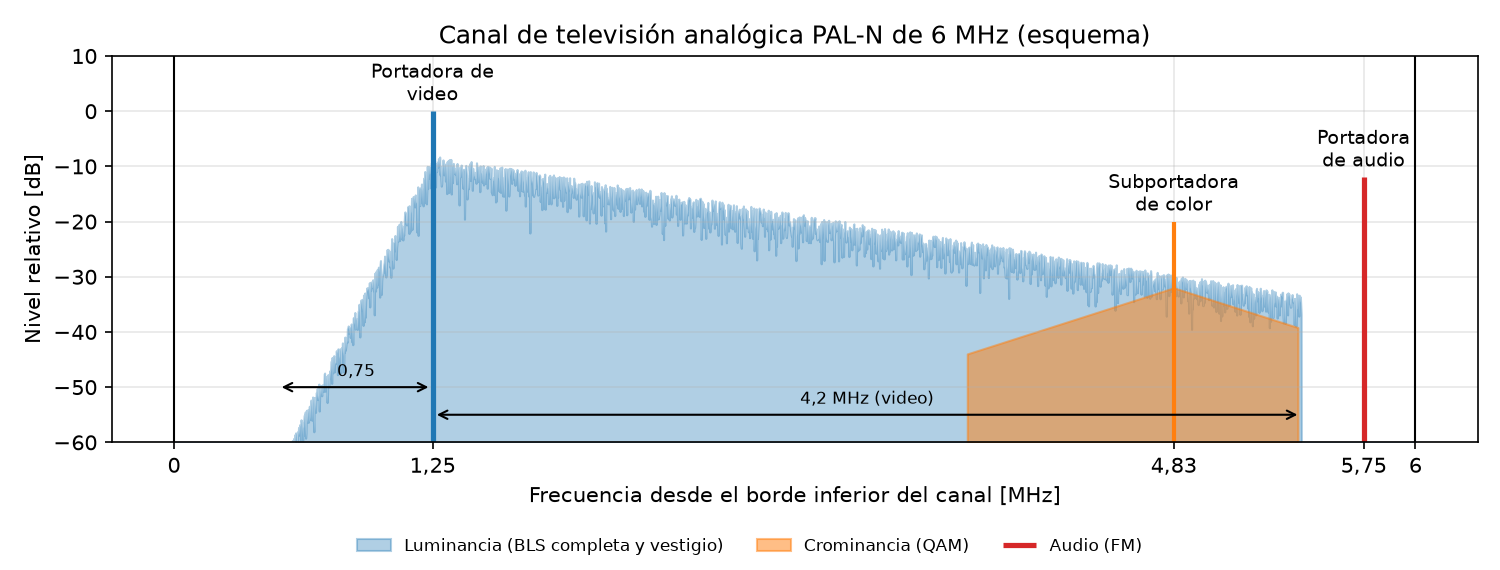
\includegraphics[width=\textwidth]{teoria/tv_pal_n.png}\\
      {\scriptsize Esquema propio a partir de la Rec. UIT-R BT.470}
    \end{column}
    \begin{column}{0.4\textwidth}
      \scriptsize
      \renewcommand{\arraystretch}{1.1}
      \setlength{\tabcolsep}{3pt}
      \begin{tabular}{ll}
        \toprule
        \textbf{Canales} & \textbf{Límite inferior [MHz]} \\
        \midrule
        2 a 4 & $54 + 6(N-2)$ \\
        5 y 6 & $76 + 6(N-5)$ \\
        7 a 13 & $174 + 6(N-7)$ \\
        21 a 51 & $512 + 6(N-21)$ \\
        \bottomrule
      \end{tabular}
      \vspace{0.2cm}

      \small
      Video en $+1{,}25$ MHz, color $+3{,}58$ MHz más arriba, audio $+4{,}5$ MHz.
    \end{column}
  \end{columns}
  \note{\textbf{Luca Baccino:} En Argentina la televisión analógica usa la norma PAL-N, con canales de 6 MHz. Los límites de cada canal salen de su número con la canalización de ENACOM: los canales 7 a 13 de VHF, por ejemplo, empiezan en 174 MHz. Los canales 52 a 69 de UHF se reasignaron a telefonía móvil en 2014, así que en UHF quedan del 21 al 51. Dentro del canal, la portadora de video está a 1,25 MHz del borde inferior, la subportadora de color 3,58 MHz más arriba y la portadora de audio a 4,5 MHz de la de video.}
\end{frame}

\begin{frame}{Canales recibidos e identificación}
  \begin{columns}[T]
    \begin{column}{0.5\textwidth}
      \centering
      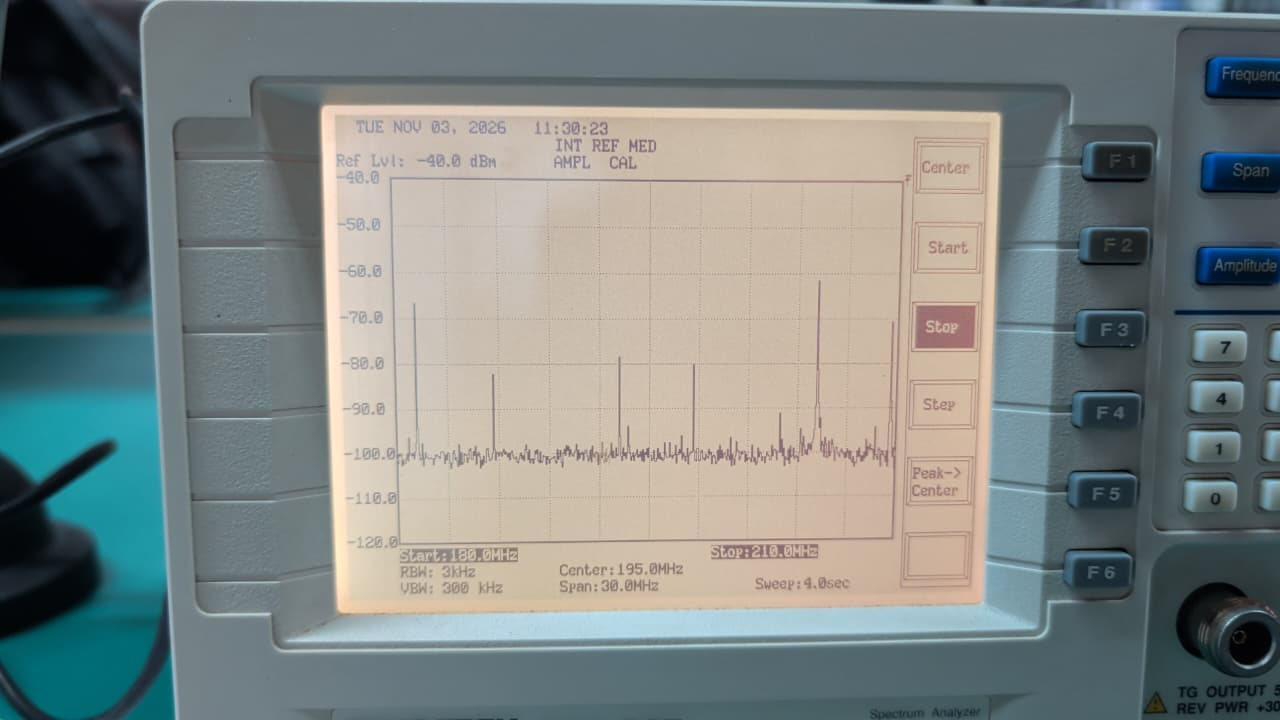
\includegraphics[width=\textwidth]{tva_vhf.png}\\
      {\scriptsize 180 a 210 MHz: canales 8, 10 y 12}
    \end{column}
    \begin{column}{0.48\textwidth}
      \scriptsize
      \renewcommand{\arraystretch}{1.15}
      \setlength{\tabcolsep}{3pt}
      \begin{tabular}{lcc}
        \toprule
        & \textbf{Canal 10} & \textbf{Canal 12} \\
        \midrule
        Límites [MHz] & 192--198 & 204--210 \\
        Video [MHz] & 193,2 & 205,2 \\
        \quad nivel [dBm] & $-75$ & $-60$ \\
        Color [MHz] & -- & 208,8 \\
        \quad nivel [dBm] & bajo el ruido & $-93$ \\
        Audio [MHz] & 197,7 & 209,7 \\
        \quad nivel [dBm] & $-85$ & $-70$ \\
        \bottomrule
      \end{tabular}
    \end{column}
  \end{columns}
  \note{\textbf{Luca Baccino:} En el tramo de 180 a 210 MHz recibimos tres canales analógicos, el 8, el 10 y el 12, que identificamos por su par de portadoras de video y audio y por la canalización. Los canales 10 y 12 los medimos en detalle, con un span de 6 MHz que abarca justo el canal. La tabla resume las tres componentes que pide la consigna: la portadora de video, la subportadora de color y la portadora de audio. La de color sólo se distingue en el canal 12, que llega unos 15 dB más fuerte; en el 10 queda en el ruido.}
\end{frame}

\begin{frame}{Componentes, ancho de banda y banda lateral vestigial}
  \begin{columns}[T]
    \begin{column}{0.49\textwidth}
      \centering
      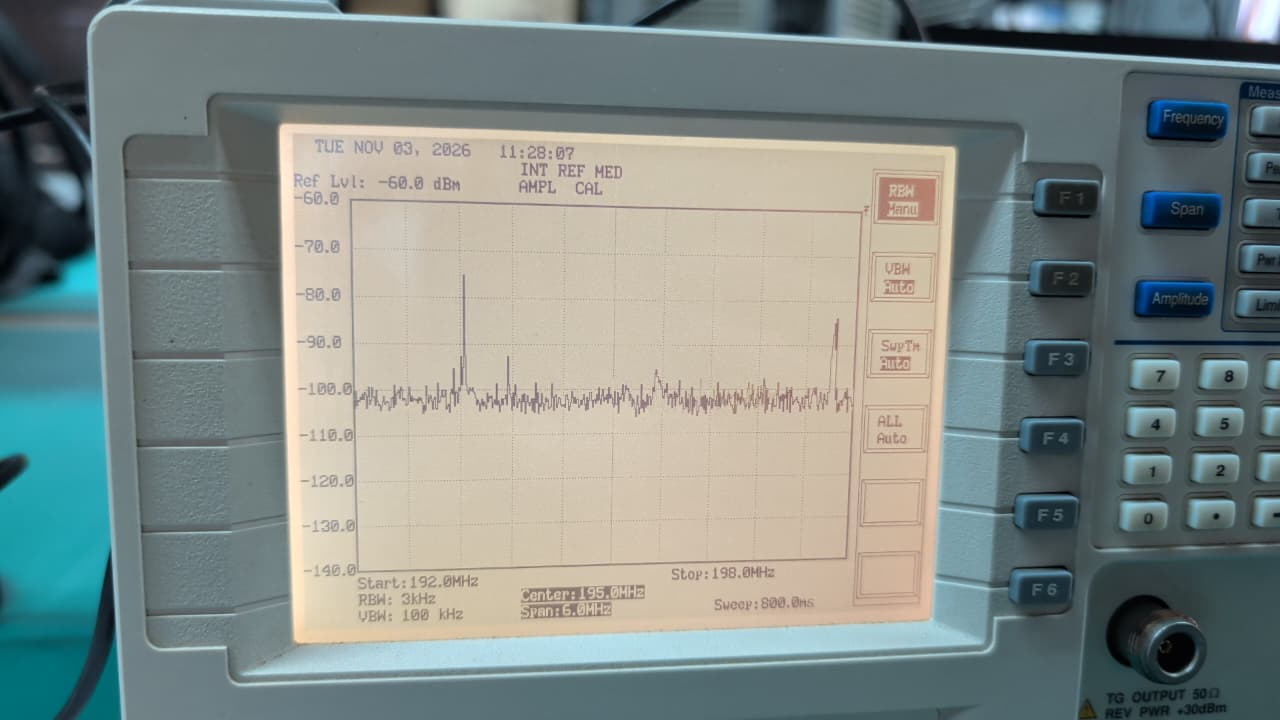
\includegraphics[width=\textwidth]{tva_canal10.png}\\
      {\scriptsize Canal 10 (192 a 198 MHz)}
    \end{column}
    \begin{column}{0.49\textwidth}
      \centering
      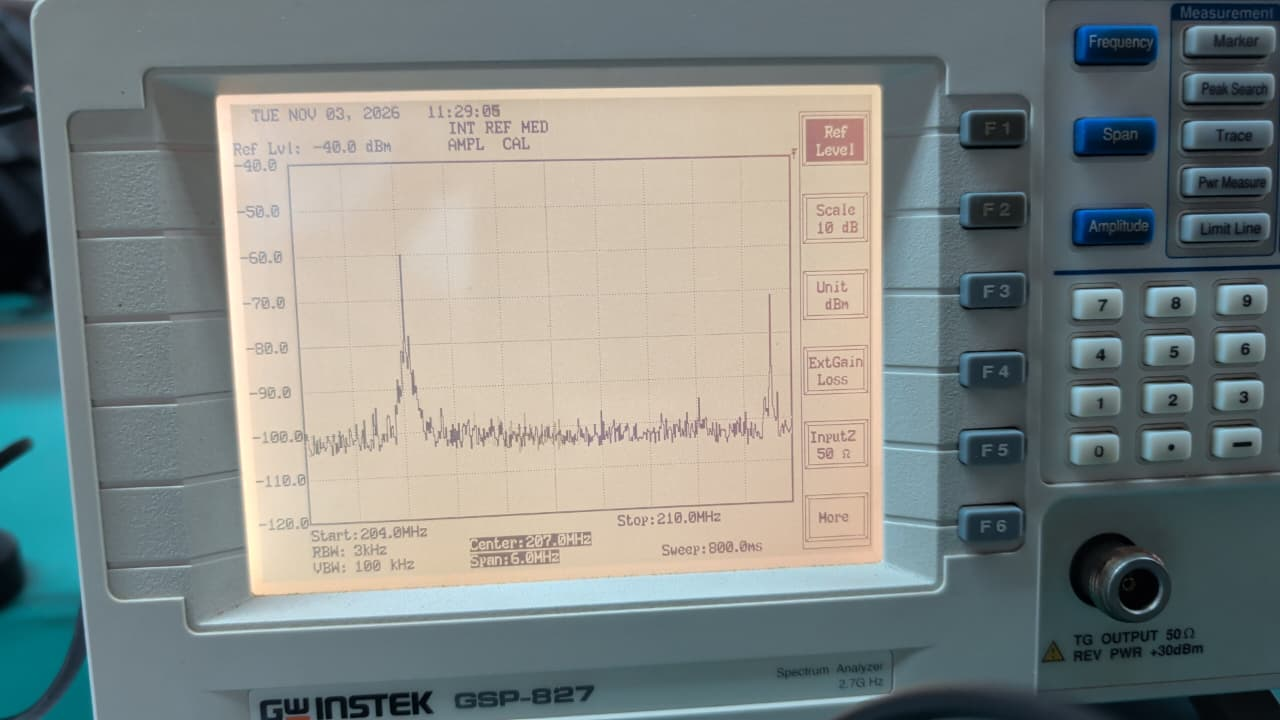
\includegraphics[width=\textwidth]{tva_canal12.png}\\
      {\scriptsize Canal 12 (204 a 210 MHz)}
    \end{column}
  \end{columns}
  \vspace{0.1cm}
  \small
  \begin{itemize}
    \item Video--audio $\approx 4{,}5$ MHz. Color en el canal 12: energía de la croma y la ráfaga
    \item Ancho de banda: video $0{,}75 + 4{,}2 \approx 5$ MHz en el canal de 6 MHz; no medible, bajo el ruido
    \item Vestigial: con DBL serían 8,4 MHz; con BLU, un filtro irrealizable
  \end{itemize}
  \note{\textbf{Luca Baccino:} En el detalle se ven las portadoras de video y audio, separadas unos 4,5 MHz como dice la norma, y en el canal 12 la subportadora de color: como está suprimida, lo que vemos es la energía de las señales de color y de la ráfaga de referencia. El video ocupa unos 5 MHz dentro del canal de 6, pero sus bandas laterales se reparten en más de 4 MHz y quedan bajo el ruido, así que el ancho de banda no lo pudimos medir. ¿Por qué banda lateral vestigial? Con doble banda lateral el video ocuparía 8,4 MHz y no entraría en el canal; con banda lateral única haría falta un filtro de corte abrupto justo en la portadora, imposible de construir sin distorsionar las bajas frecuencias. El vestigio es el compromiso.}
\end{frame}

\begin{frame}{Audio y video, canales adyacentes y síntesis}
  \small
  \begin{block}{Nivel del audio respecto del video}
    $\approx -10$ dB en los dos canales, como se transmite normalmente.\\
    Condiciones: \textit{span} 6 MHz, RBW 3 kHz, VBW 100 kHz. Con modulación negativa, el nivel de la portadora de video depende del brillo de la imagen.
  \end{block}
  \begin{block}{Canales adyacentes}
    Se reciben 8, 10 y 12; los canales 9 y 11 están libres: en una zona no se asignan canales contiguos por aire.
  \end{block}
  \begin{block}{Síntesis}
    Video: AM con banda lateral vestigial y modulación negativa. Color: QAM sobre subportadora, fase alternada por línea. Audio: FM, $\pm 25$ kHz.
  \end{block}
  \note{\textbf{Luca Baccino:} La portadora de audio quedó unos 10 dB por debajo de la de video en los dos canales, que es la relación con que se transmite normalmente. La consigna pide las condiciones: medimos con un span de 6 MHz y un RBW de 3 kHz, y hay que tener en cuenta que, con modulación negativa, el nivel de la portadora de video cambia con el brillo de la imagen, mientras que el audio en FM es constante. En cuanto a los adyacentes, sólo se reciben el 8, el 10 y el 12, con el 9 y el 11 libres, porque el audio de un canal queda muy cerca del vestigio del siguiente. En síntesis, cada componente usa una modulación distinta: AM vestigial para el video, cuadratura para el color y FM para el audio.}
\end{frame}

% =====================================================
\section[TDA]{Televisión digital (TDA)}
\orador{Vuelta 1}{Luca Baccino}
\begin{frame}{Exploración e identificación: canal 27}
  \begin{columns}[T]
    \begin{column}{0.55\textwidth}
      \centering
      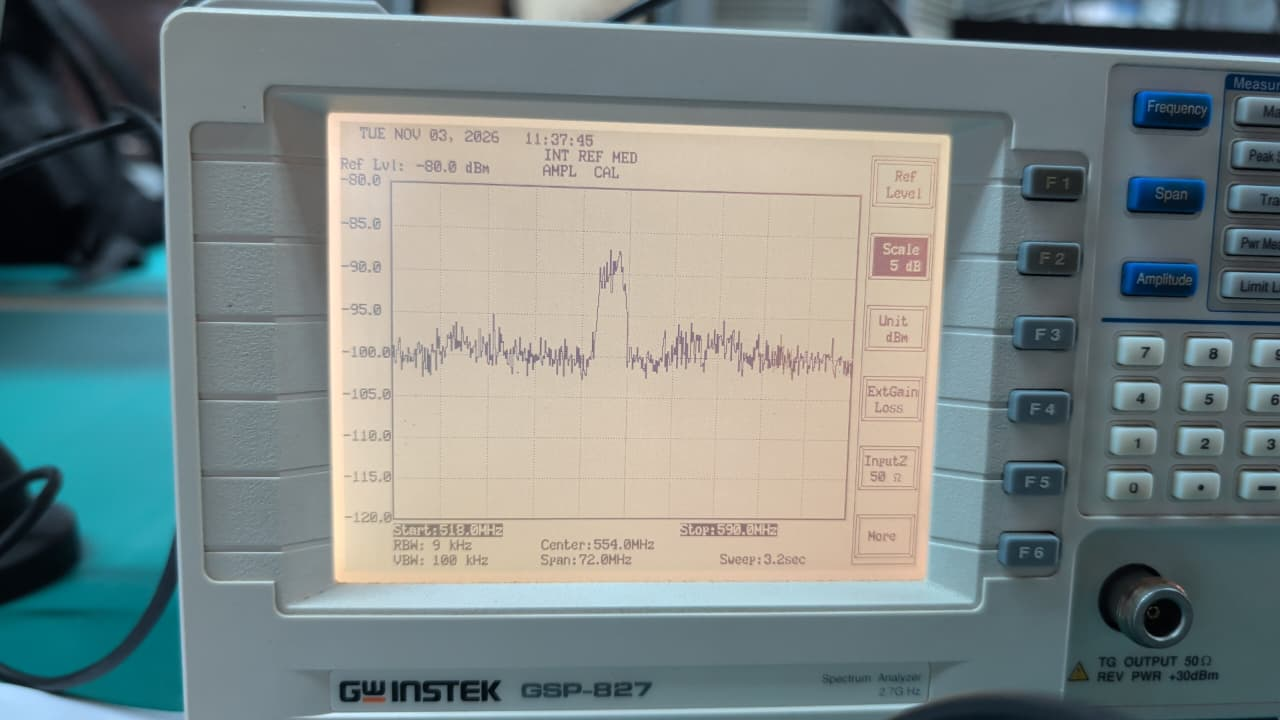
\includegraphics[width=\textwidth]{tda_canal.png}\\
      {\scriptsize 518 a 590 MHz (canales 22 a 33), RBW 9 kHz}
    \end{column}
    \begin{column}{0.43\textwidth}
      \small
      \begin{itemize}
        \item Un canal claramente sobre el ruido: 549,5 a 555 MHz
        \item $f_{inf} = 512 + 6(N - 21)$ $\Rightarrow$ \textbf{canal 27} (548 a 554 MHz)
        \item El corrimiento de $\approx 1$ MHz está dentro del error de lectura
        \item A los lados, el piso sube 2 a 3 dB: posibles canales débiles
      \end{itemize}
    \end{column}
  \end{columns}
  \note{\textbf{Luca Baccino:} En la televisión digital exploramos de 518 a 590 MHz, que abarca los canales 22 a 33. Apareció un canal claramente por encima del ruido, entre unos 549,5 y 555 MHz. Con la fórmula de la canalización corresponde al canal 27, de 548 a 554; el corrimiento de alrededor de 1 MHz está dentro del error de leer sobre la grilla, que tiene divisiones de 7,2 MHz. A los costados el piso se eleva un poco, lo que podría ser otros canales digitales que llegan demasiado débiles para distinguirlos.}
\end{frame}

\begin{frame}{Ancho de banda, forma OFDM y potencia de canal}
  \small
  \begin{columns}[T]
    \begin{column}{0.5\textwidth}
      \begin{block}{Ancho de banda}
        Criterio: flancos de la meseta ($-3$ dB).\\
        Medido $\approx 5{,}5$ MHz; teórico 5,57 MHz (13 segmentos), en el canal nominal de 6 MHz.
      \end{block}
      \begin{block}{Forma del espectro}
        Meseta plana y flancos abruptos: miles de subportadoras de igual nivel que el RBW no resuelve. Sin portadora destacada.
      \end{block}
    \end{column}
    \begin{column}{0.48\textwidth}
      \begin{block}{Potencia de canal}
        Meseta $\approx -89$ dBm, piso $\approx -100$ dBm
        \[ P \approx -89 + 10\log\frac{5{,}57\text{ MHz}}{9\text{ kHz}} \]
        \[ P \approx -61 \text{ dBm} \]
      \end{block}
    \end{column}
  \end{columns}
  \note{\textbf{Luca Baccino:} El ancho de banda de una señal OFDM se mide entre los flancos de la meseta. Medimos unos 5,5 MHz, coherente con los 5,57 de la norma, que son los 13 segmentos, dentro del canal nominal de 6 MHz. La forma es típica de OFDM: una meseta plana, porque las subportadoras tienen todas el mismo nivel y están tan juntas que el analizador no las resuelve, con flancos abruptos y sin ninguna portadora destacada, a diferencia de la analógica. Para el nivel no sirve leer el pico: hay que integrar la densidad en todo el ancho, y da una potencia de canal de unos menos 61 dBm.}
\end{frame}

\begin{frame}{Recepción con televisor y síntesis de ISDB-Tb}
  \small
  \begin{block}{Búsqueda de canales con un receptor}
    No se realizó: no se dispuso de un televisor o receptor ISDB-Tb en el laboratorio, por lo que no se compararon las señales con los servicios decodificados.
  \end{block}
  La presencia en el analizador no garantiza la recepción: hace falta nivel sobre la sensibilidad, C/N suficiente para cada capa (mayor en 64-QAM que en QPSK), ecos dentro del intervalo de guarda y ausencia de interferencias. Meseta a $\approx 11$ dB del piso del analizador: margen reducido.
  \begin{block}{Síntesis}
    ISDB-Tb: OFDM en 13 segmentos agrupados en hasta tres capas (DQPSK, QPSK, 16-QAM, 64-QAM). Un canal lleva HD fijo y \textit{one-seg} móvil.
  \end{block}
  \note{\textbf{Luca Baccino:} La consigna pedía conectar la antena a un televisor, buscar canales y comparar. No pudimos hacerlo porque no tuvimos un receptor disponible, y lo dejamos indicado. Lo que sí podemos decir es que ver la señal en el analizador no garantiza recibirla: el receptor necesita nivel suficiente, una relación portadora a ruido que alcance para la modulación de cada capa, que los ecos caigan dentro del intervalo de guarda y que no haya interferencias. La meseta quedó unos 11 dB sobre el piso del analizador, un margen reducido, aunque el ruido de un televisor suele ser menor. En síntesis, ISDB-Tb usa OFDM en 13 segmentos agrupados en capas, lo que permite llevar en un canal un programa en alta definición y uno para móviles. El detalle del sistema lo desarrolla Agustín en la segunda vuelta, que arranca Cristian.}
\end{frame}

% =====================================================
\section[Niveles]{Niveles y ejercicio}
\orador{Vuelta 2}{Cristian Arteaga Barrera}
\begin{frame}{Unidades: dBm, dBµV y dBc}
  \begin{columns}[T]
    \begin{column}{0.5\textwidth}
      \small
      \begin{block}{dBm: potencia absoluta}
        $P_{dBm} = 10\log(P / 1\text{ mW})$\\
        $0$ dBm $= 1$ mW; $-30$ dBm $= 1$ µW
      \end{block}
      \begin{block}{dBµV: tensión absoluta}
        $V_{dB\mu V} = 20\log(V / 1\text{ µV})$
      \end{block}
    \end{column}
    \begin{column}{0.48\textwidth}
      \small
      \begin{block}{dBc: relativo a la portadora}
        $N_{dBc} = N_{comp} - N_{portadora}$\\
        No depende de la impedancia ni de la ganancia del sistema.
      \end{block}
      Se usa para bandas laterales, espurias y armónicas.
    \end{column}
  \end{columns}
  \note{\textbf{Cristian Arteaga Barrera:} Arrancamos la segunda vuelta con la Parte 2, los niveles. El dBm es una medida absoluta de potencia respecto de un miliwatt: cero dBm es un miliwatt, menos 30 es un microwatt. El dBµV es una medida absoluta de tensión respecto de un microvolt; como es un cociente de tensiones, lleva 20 por el logaritmo. Y el dBc es relativo: la diferencia entre el nivel de una componente y el de la portadora. Por eso no depende ni de la impedancia ni de la ganancia, y es el que se usa para las bandas laterales, como en AM.}
\end{frame}

\begin{frame}{Potencia y tensión: por qué importa la impedancia}
  \begin{columns}[T]
    \begin{column}{0.5\textwidth}
      \small
      \[ P = \frac{V^2}{R} \;\Rightarrow\; V_{dB\mu V} = P_{dBm} + 90 + 10\log R \]
      \renewcommand{\arraystretch}{1.15}
      \begin{tabular}{lcc}
        \toprule
        & $50\,\Omega$ & $75\,\Omega$ \\
        \midrule
        dBµV & dBm $+ 107{,}0$ & dBm $+ 108{,}8$ \\
        $-20$ dBm & 22,4 mV & 27,4 mV \\
        $-60$ dBm & 224 µV & 274 µV \\
        \bottomrule
      \end{tabular}
    \end{column}
    \begin{column}{0.48\textwidth}
      \small
      \begin{itemize}
        \item 1 mV entrega $-47$ dBm sobre $50\,\Omega$ y $-48{,}8$ dBm sobre $75\,\Omega$
        \item Sin la impedancia, la conversión es ambigua en \textbf{1,76 dB}
        \item Caso típico: medir una red de $75\,\Omega$ (dBµV) con un analizador de $50\,\Omega$ (dBm)
      \end{itemize}
    \end{column}
  \end{columns}
  \note{\textbf{Cristian Arteaga Barrera:} Para pasar de potencia a tensión se usa P igual a V cuadrado sobre R, así que la conversión depende de la resistencia. Desarrollando, el nivel en dBµV es el nivel en dBm más 90 más diez logaritmo de R: en 50 ohms se suman 107 dB y en 75 ohms, 108,8. Por ejemplo, un milivolt sobre 50 ohms son menos 47 dBm, y sobre 75 ohms, menos 48,8. Si no se dice la impedancia, la conversión es ambigua en 1,76 dB. Es justamente lo que pasa al medir una red de televisión de 75 ohms, cuyos niveles se dan en dBµV, con un analizador de 50 ohms que mide en dBm.}
\end{frame}

\begin{frame}{Ejercicio: índice de modulación de una señal AM}
  \small
  Portadora $-20$ dBm, bandas laterales $-60$ dBm, sobre $50\,\Omega$.
  \begin{columns}[T]
    \begin{column}{0.5\textwidth}
      \begin{block}{En tensión}
        \[ E_c = \sqrt{10^{-5}\cdot 50} = 22{,}36 \text{ mV} \]
        \[ E_{BL} = \sqrt{10^{-9}\cdot 50} = 0{,}2236 \text{ mV} \]
        \[ m = \frac{2E_{BL}}{E_c} = 0{,}02 \]
      \end{block}
    \end{column}
    \begin{column}{0.48\textwidth}
      \begin{block}{En dBc}
        \[ N_{BL} - N_c = -40 \text{ dBc} \]
        \[ m = 2\cdot 10^{-40/20} = 0{,}02 \]
      \end{block}
      \centering
      \Large\textbf{$m = 2$ \%}
    \end{column}
  \end{columns}
  \vspace{0.1cm}
  La impedancia se cancela en el cociente. Las BL llevan sólo el 0,02 \% de la potencia de la portadora.
  \note{\textbf{Cristian Arteaga Barrera:} El ejercicio pide el índice de modulación de una AM con portadora de menos 20 dBm y bandas laterales de menos 60. Pasando a tensión sobre 50 ohms, la portadora es de 22,36 milivolts y cada banda lateral de 0,2236. Como cada banda lateral vale m sobre dos por la portadora, m da 0,02, o sea un 2 por ciento. Más directo es usar la diferencia: menos 40 dBc da el mismo resultado. Y en 75 ohms cambian las tensiones pero no su cociente. Es una modulación muy débil: las bandas laterales llevan apenas el 0,02 por ciento de la potencia de la portadora.}
\end{frame}

% =====================================================
\section[DVB-C y DOCSIS]{DVB-C y DOCSIS}
\orador{Vuelta 2}{Cristian Arteaga Barrera}
\begin{frame}{DVB-C}
  \begin{columns}[T]
    \begin{column}{0.5\textwidth}
      \small
      \begin{block}{Red y modulación}
        \begin{itemize}
          \item ETSI EN 300 429; UIT-T J.83, Anexo A
          \item Redes de cable coaxial y HFC: canal benigno, SNR $> 30$ dB
          \item QAM de portadora única: 16 a 256 estados
          \item Diseñado para 8 MHz; se adapta a 6 MHz
        \end{itemize}
      \end{block}
    \end{column}
    \begin{column}{0.48\textwidth}
      \small
      \begin{block}{Transporte de los servicios}
        Flujo de transporte MPEG-2 (paquetes de 188 bytes) con varios programas y tablas PAT, PMT, NIT, SDT, EIT. Pagos: acceso condicional.
      \end{block}
      \setbeamercolor{block title}{bg=grupo oeste,fg=white}
      \setbeamercolor{block body}{bg=grupo oeste!8}
      \begin{block}{En Argentina}
        Cablevisión (Flow, 2017): decodificador híbrido ARRIS DCX4220, QAM + IP.\\
        {\scriptsize Fuente: Lightwave Online.}
      \end{block}
    \end{column}
  \end{columns}
  \note{\textbf{Cristian Arteaga Barrera:} En la Parte 3, DVB-C es la norma de televisión digital por cable, la EN 300 429 de ETSI, que la UIT recoge en el Anexo A de la J.83. Se usa en redes de cable coaxial e híbridas fibra-coaxial, que son un canal mucho más benigno que el aire: sin multitrayecto severo y con más de 30 dB de relación señal a ruido. Por eso usa QAM de una sola portadora, de 16 a 256 estados. Los programas viajan en un flujo de transporte MPEG-2, con tablas que indican qué paquetes forman cada programa, y los pagos se cifran con acceso condicional. Un ejemplo en Argentina es Cablevisión, que en 2017 desplegó para Flow un decodificador híbrido que recibe tanto los canales QAM como contenido IP; la fuente es Lightwave.}
\end{frame}

\begin{frame}{DOCSIS: función, equipos y sentidos de transmisión}
  \centering
  \resizebox{\textwidth}{!}{%
    \begin{tikzpicture}[node distance=1.1cm, every node/.style={font=\small},
        caja/.style={draw, rounded corners, minimum height=1cm, minimum width=2.2cm, align=center, fill=blue!6}]
        \node[caja, fill=orange!12] (inet) {Internet /\\red IP};
        \node[caja, right=of inet] (cmts) {CMTS};
        \node[caja, below=0.6cm of cmts] (video) {Cabecera de\\video (QAM)};
        \node[caja, right=1.3cm of cmts] (comb) {Combinador\\RF};
        \node[caja, right=1.3cm of comb] (tx) {Transmisor y\\receptor óptico};
        \node[caja, right=1.6cm of tx] (nodo) {Nodo\\óptico};
        \node[caja, right=1.3cm of nodo] (amp) {Amplificador\\y \textit{taps}};
        \node[caja, above right=0.2cm and 1.0cm of amp, fill=green!8] (cm) {Cable\\módem};
        \node[caja, below right=0.2cm and 1.0cm of amp, fill=green!8] (stb) {Decodificador\\o TV};
        \draw[{Stealth}-{Stealth}] (inet) -- (cmts);
        \draw[{Stealth}-{Stealth}] (cmts) -- (comb);
        \draw[-{Stealth}] (video) -| (comb);
        \draw[{Stealth}-{Stealth}] (comb) -- (tx);
        \draw[{Stealth}-{Stealth}, very thick, red!70!black] (tx) -- node[above]{fibra} (nodo);
        \draw[{Stealth}-{Stealth}, very thick] (nodo) -- node[above]{coaxial} (amp);
        \draw[{Stealth}-{Stealth}] (amp.east) -- (cm.west);
        \draw[-{Stealth}] (amp.east) -- (stb.west);
        \node[draw, dashed, fit=(cmts)(video)(comb)(tx), inner sep=6pt, label=above:{Cabecera}] {};
    \end{tikzpicture}}
  \vspace{0.2cm}

  \raggedright\small
  \begin{itemize}
    \item Agrega a la red de cable un canal de datos bidireccional (CableLabs; UIT-T J.222)
    \item \textbf{Descendente:} el CMTS difunde a todos los módems (QAM; OFDM desde 3.1)
    \item \textbf{Ascendente:} medio compartido; los módems transmiten en turnos que asigna el CMTS
  \end{itemize}
  \note{\textbf{Cristian Arteaga Barrera:} DOCSIS es la familia de especificaciones de CableLabs, adoptada por la UIT, que le agrega a la red de cable un canal de datos bidireccional. Los equipos principales son el CMTS, en la cabecera, que modula los canales de bajada, recibe los de subida y administra el acceso, y el cable módem en la casa del abonado; entre ellos está la red híbrida de fibra hasta el nodo y coaxial con amplificadores y derivadores. En sentido descendente el CMTS difunde a todos los módems del nodo. En sentido ascendente el medio es compartido, así que cada módem transmite en los intervalos que le asigna el CMTS.}
\end{frame}

\begin{frame}{DOCSIS: versiones, Internet y video sobre IP}
  \begin{columns}[T]
    \begin{column}{0.56\textwidth}
      \scriptsize
      \renewcommand{\arraystretch}{1.15}
      \setlength{\tabcolsep}{3pt}
      \begin{tabular}{cccl}
        \toprule
        \textbf{Versión} & \textbf{Bajada} & \textbf{Subida} & \textbf{Novedad} \\
        \midrule
        1.0 (1997) & 40 Mbps & 10 Mbps & Primer estándar \\
        2.0 (2001) & 40 Mbps & 30 Mbps & A-TDMA, S-CDMA \\
        3.0 (2006) & 1 Gbps & 200 Mbps & Agregación de canales \\
        3.1 (2013) & 10 Gbps & 1--2 Gbps & OFDM, 4096-QAM \\
        4.0 (2017) & 10 Gbps & 6 Gbps & 1,8 GHz, \textit{full duplex} \\
        \bottomrule
      \end{tabular}
    \end{column}
    \begin{column}{0.42\textwidth}
      \small
      \begin{itemize}
        \item Tecnología de acceso a Internet de las redes de cable: cada módem recibe una IP
        \item Video sobre IP: IPTV gestionada y OTT por el módem
        \item Migración a todo IP: el espectro de video QAM pasa a DOCSIS
      \end{itemize}
    \end{column}
  \end{columns}
  \note{\textbf{Cristian Arteaga Barrera:} La familia fue creciendo: DOCSIS 3.0 agregó la agregación de canales y llegó a un gigabit; la 3.1 incorporó OFDM, con constelaciones de hasta 4096-QAM, y alcanza unos 10 gigabits de bajada; la 4.0 extiende el espectro a 1,8 GHz y permite full duplex. La relación con Internet es directa: DOCSIS es el acceso a Internet de las redes de cable, y el CMTS funciona como un router. Y como transporta IP, también lleva video: IPTV y plataformas OTT por el mismo módem. A medida que los operadores apagan los canales de video QAM, ese espectro pasa a DOCSIS y toda la televisión se entrega por IP. Le paso a Joaquín.}
\end{frame}

% =====================================================
\section[RF Overlay]{Video RF Overlay}
\orador{Vuelta 2}{Joaquín Monja}
\begin{frame}{RF Overlay: qué es e integración con los datos}
  \small
  \begin{block}{En qué consiste}
    El espectro de RF de una red de cable (canales de 6 MHz de 47 a 1000 MHz) modula en intensidad un láser de \textbf{1550 nm}, viaja por la misma ODN de la PON y un receptor óptico lo devuelve a RF en la casa. Para el televisor es igual a una red de cable.
  \end{block}
  \begin{block}{Integración con los datos (WDM)}
    \begin{itemize}
      \item Cabecera: un combinador WDM une el video (1550 nm) con la OLT (1490 / 1310 nm)
      \item ODN: fibra, divisores y acometidas pasivos llevan las tres longitudes de onda
      \item Abonado: un filtro separa 1550 nm hacia el receptor de video
    \end{itemize}
    Servicios independientes: el video no consume capacidad de GPON.
  \end{block}
  \note{\textbf{Joaquín Monja:} El RF Overlay distribuye televisión por una red FTTH superponiendo, en una longitud de onda propia, el mismo espectro de RF que circula por una red de cable. Ese espectro modula en intensidad un láser de 1550 nanómetros, viaja por la misma fibra y los mismos divisores que los datos, y en la casa un receptor óptico lo convierte de nuevo en RF. Se integra con los datos por multiplexación en longitud de onda: en la cabecera un combinador une el video con la OLT, que transmite en 1490 y recibe en 1310; la red pasiva lleva las tres longitudes de onda; y en el abonado un filtro separa el video. Los dos servicios son independientes: el video no le quita capacidad a GPON.}
\end{frame}

\begin{frame}{Diagrama en bloques de una red FTTH con RF Overlay}
  \centering
  \resizebox{!}{0.86\textheight}{%
    \begin{tikzpicture}[every node/.style={font=\small},
        caja/.style={draw, rounded corners, minimum height=1.15cm, minimum width=2.7cm, align=center, fill=blue!6},
        int/.style={draw, fill=white, align=center, minimum width=2.4cm, minimum height=0.8cm},
        opt/.style={very thick, red!70!black}, rf/.style={thick, blue!60!black}, dat/.style={thick, green!55!black}]
        \node[caja, fill=orange!12] (fuentes) at (0, 0) {Satélite, fibra\\y señales locales};
        \node[caja] (cab) at (3.7, 0) {Cabecera RF\\(moduladores\\QAM o ISDB-Tb)};
        \node[caja] (txo) at (7.4, 0) {Transmisor óptico\\$1.550 \, nm$};
        \node[caja] (edfa) at (11.1, 0) {Amplificador\\óptico EDFA};
        \node[caja, fill=orange!12] (red) at (0, -2.4) {Red IP /\\enlace mayorista};
        \node[caja] (olt) at (3.7, -2.4) {OLT GPON\\$1.490 / 1.310 \, nm$};
        \node[caja] (wdm) at (11.1, -2.4) {Combinador\\WDM};
        \node[caja] (spl) at (11.1, -4.8) {Divisores ópticos\\$1{:}4$ y $1{:}16$};
        \node[int] (rxv) at (11.1, -8.0) {Receptor de\\video $1.550$};
        \node[int] (ontd) at (11.1, -9.2) {ONT de datos};
        \node[font=\small\bfseries] (ontlab) at (11.1, -7.2) {ONT con CATV};
        \node[draw, rounded corners, fill=green!8, fit=(ontlab)(rxv)(ontd), inner sep=5pt] (ont) {};
        \node[font=\small\bfseries] at (11.1, -7.2) {ONT con CATV};
        \node[int] (rxv) at (11.1, -8.0) {Receptor de\\video $1.550$};
        \node[int] (ontd) at (11.1, -9.2) {ONT de datos};
        \node[caja, fill=yellow!12] (tv) at (6.4, -8.0) {Televisores\\(coaxial $75 \, \Omega$)};
        \node[caja, fill=yellow!12] (lan) at (6.4, -9.4) {Router, Wi-Fi\\y STB IPTV};
        \draw[-{Stealth}] (fuentes) -- (cab);
        \draw[-{Stealth}, rf] (cab) -- node[above, font=\scriptsize]{RF} (txo);
        \draw[-{Stealth}, opt] (txo) -- node[above, font=\scriptsize]{$1.550$} (edfa);
        \draw[-{Stealth}, opt] (edfa) -- (wdm);
        \draw[{Stealth}-{Stealth}, dat] (red) -- (olt);
        \draw[{Stealth}-{Stealth}, opt] (olt) -- node[above, font=\scriptsize]{$1.490 / 1.310$} (wdm);
        \draw[{Stealth}-{Stealth}, opt] (wdm) -- node[right, font=\scriptsize]{fibra troncal ($3 \, \lambda$)} (spl);
        \draw[{Stealth}-{Stealth}, opt] (spl) -- node[pos=0.4, right, font=\scriptsize]{acometida} (ont);
        \draw[-{Stealth}, rf] (rxv) -- node[above, font=\scriptsize]{RF} (tv);
        \draw[{Stealth}-{Stealth}, dat] (ontd.west) -- node[above, font=\scriptsize]{Ethernet} (lan.east |- ontd.west);
        \node[draw, dashed, fit=(cab)(edfa)(olt)(wdm), inner sep=8pt, label={[font=\small]above:Oficina central / cabecera}] {};
        \node[draw, dashed, fit=(spl), inner sep=8pt, label={[font=\small]left:ODN}] {};
        \node[draw, dashed, fit=(ont)(tv)(lan), inner sep=8pt, label={[font=\small]below:Domicilio del abonado}] {};
    \end{tikzpicture}}
  \note{\textbf{Joaquín Monja:} Este es el diagrama en bloques que pide la consigna. Arriba, la cabecera de video reúne los canales y los modula; el transmisor óptico los pasa a 1550 nanómetros y el amplificador EDFA les da potencia. Abajo, la OLT de GPON conecta la red de datos. El combinador WDM junta las dos señales en la fibra troncal, que pasa por los divisores de la red de distribución hasta la casa del abonado. Ahí, la ONT con salida de televisión separa el video, que sale por coaxial a los televisores, y los datos, que salen por Ethernet al router.}
\end{frame}

\begin{frame}{Componentes y longitudes de onda}
  \begin{columns}[T]
    \begin{column}{0.56\textwidth}
      \scriptsize
      \begin{itemize}
        \item \textbf{Transmisor óptico 1550 nm:} pasa el espectro de RF a intensidad del láser; muy lineal para evitar intermodulación
        \item \textbf{EDFA:} amplifica en el dominio óptico; compensa la división (1:64 $\approx$ 25 dB)
        \item \textbf{Combinador WDM:} une video y PON con baja pérdida y buen aislamiento
        \item \textbf{ODN:} la misma red pasiva de la red de datos
        \item \textbf{Receptor de video:} fotodiodo y amplificador de RF de bajo ruido
      \end{itemize}
    \end{column}
    \begin{column}{0.42\textwidth}
      \centering
      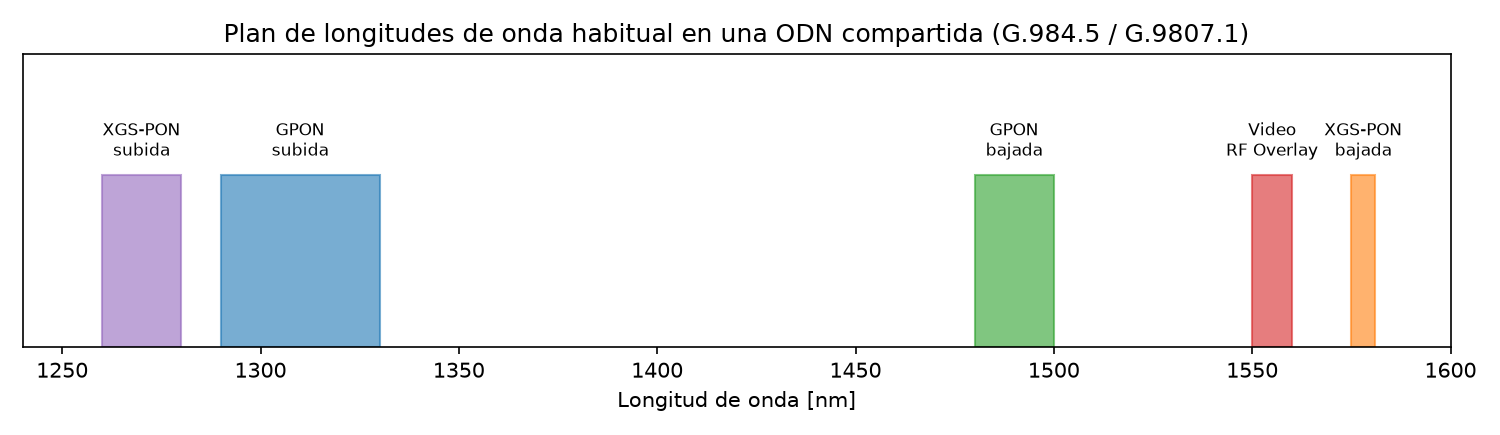
\includegraphics[width=\textwidth]{teoria/longitudes_onda.png}\\[0.1cm]
      \scriptsize
      \raggedright
      GPON 1490/1310 nm; video 1550--1560 nm; XGS-PON 1577/1270 nm. Pueden variar según la arquitectura.
    \end{column}
  \end{columns}
  \note{\textbf{Joaquín Monja:} Las funciones de cada componente: el transmisor óptico convierte el espectro de RF en variaciones de intensidad del láser, y tiene que ser muy lineal, porque lleva muchos canales a la vez y cualquier no linealidad produce intermodulación. El amplificador EDFA amplifica directamente la luz y compensa la atenuación de la división, que en una red 1 a 64 es de unos 25 dB. El combinador WDM une las longitudes de onda con poca pérdida. La red de distribución es la misma de los datos, y el receptor de video es un fotodiodo con un amplificador de bajo ruido. En cuanto a las longitudes de onda: GPON usa 1490 de bajada y 1310 de subida, el video 1550 a 1560, y XGS-PON 1577 y 1270; pueden variar según la arquitectura.}
\end{frame}

\begin{frame}{Llegada al televisor y comparación con IPTV}
  \small
  \textbf{Al televisor:} el receptor óptico entrega por coaxial de $75\,\Omega$ el mismo espectro de la cabecera; con divisores de RF llega a cada aparato, que sintoniza PAL-N, ISDB-Tb o DVB-C.
  \vspace{0.15cm}

  \centering
  \renewcommand{\arraystretch}{1.15}
  \begin{tabular}{p{2.2cm}>{\raggedright\arraybackslash}p{4.6cm}>{\raggedright\arraybackslash}p{4.6cm}}
    \toprule
    & \textbf{RF Overlay} & \textbf{IPTV} \\
    \midrule
    Transporte & Espectro de RF completo en 1550 nm & Paquetes IP multicast en la bajada de la PON \\
    Distribución & Difusión: todos los canales a todos & Sólo los canales que se miran \\
    Recepción & Sintonizador del TV, por coaxial & STB o aplicación, por HDMI o Wi-Fi \\
    \bottomrule
  \end{tabular}
  \note{\textbf{Joaquín Monja:} Para llegar al televisor, el receptor óptico entrega por coaxial el mismo espectro que sale de la cabecera, y con divisores de RF se reparte a cada aparato, como en una instalación de cable común. El televisor sintoniza con su propio sintonizador. La alternativa es la IPTV, donde cada canal es un flujo IP multicast que viaja por la red de datos: la OLT envía cada canal una sola vez por puerto PON, sólo si algún abonado lo pidió, y un decodificador lo convierte para el televisor. La diferencia de fondo es que el RF Overlay difunde todo a todos y la IPTV transporta sólo lo que se mira.}
\end{frame}

\begin{frame}{Ventajas, limitaciones y condiciones de aplicación}
  \centering
  \scriptsize
  \renewcommand{\arraystretch}{1.15}
  \begin{tabular}{p{2.2cm}>{\raggedright\arraybackslash}p{4.8cm}>{\raggedright\arraybackslash}p{4.8cm}}
    \toprule
    & \textbf{RF Overlay} & \textbf{IPTV} \\
    \midrule
    Ventajas & Sin decodificador; no carga la red de datos; cambio de canal inmediato; facilita migrar abonados HFC & Una sola red IP; interactividad (video a pedido, grabación en red); canales casi ilimitados \\
    \midrule
    Limitaciones & Equipamiento óptico lineal y potente, costoso; presupuesto óptico propio; sin interactividad & Un STB o aplicación por pantalla; consume capacidad; exige multicast, IGMP y QoS; sensible a la congestión \\
    \midrule
    Conviene cuando & Hay muchos abonados de cable con televisores sin decodificador, una grilla lineal amplia o poca capacidad de datos & Se diseña una red nueva con margen de capacidad \\
    \bottomrule
  \end{tabular}
  \note{\textbf{Joaquín Monja:} El RF Overlay funciona con cualquier televisor sin decodificador, no carga la red de datos y facilita migrar a los abonados de una red de cable, pero necesita equipamiento óptico de video, lineal y potente, que es caro, y no tiene interactividad. La IPTV usa una sola red y permite video a pedido y grabación en red, pero necesita un decodificador o una aplicación por pantalla, consume capacidad y exige una red con multicast y calidad de servicio bien configuradas. Por eso el RF Overlay conviene cuando hay una base grande de abonados de cable con televisores comunes, y la IPTV es la opción natural en una red nueva con capacidad de sobra. Sigue Agustín.}
\end{frame}

% =====================================================
\section[ISDB-Tb]{ISDB-Tb}
\orador{Vuelta 2}{Agustín Mendes Rosa}
\begin{frame}{ISDB-Tb: principio de OFDM}
  \begin{columns}[T]
    \begin{column}{0.5\textwidth}
      \small
      \begin{itemize}
        \item Norma de la TDA (2009): ISDB-T japonés con H.264, AAC y Ginga
        \item Miles de subportadoras lentas, separadas $\Delta f = 1/T_u$: ortogonales
        \item Intervalo de guarda ($1/4$ a $1/32$ de $T_u$): los ecos dentro de él no causan interferencia entre símbolos
      \end{itemize}
      \vspace{0.1cm}
      \scriptsize
      \renewcommand{\arraystretch}{1.1}
      \begin{tabular}{cccc}
        \toprule
        \textbf{Modo} & \textbf{FFT} & \textbf{Subport.} & \textbf{$T_u$} \\
        \midrule
        1 & 2k & 1405 & 252 µs \\
        2 & 4k & 2809 & 504 µs \\
        3 & 8k & 5617 & 1008 µs \\
        \bottomrule
      \end{tabular}
    \end{column}
    \begin{column}{0.48\textwidth}
      \centering
      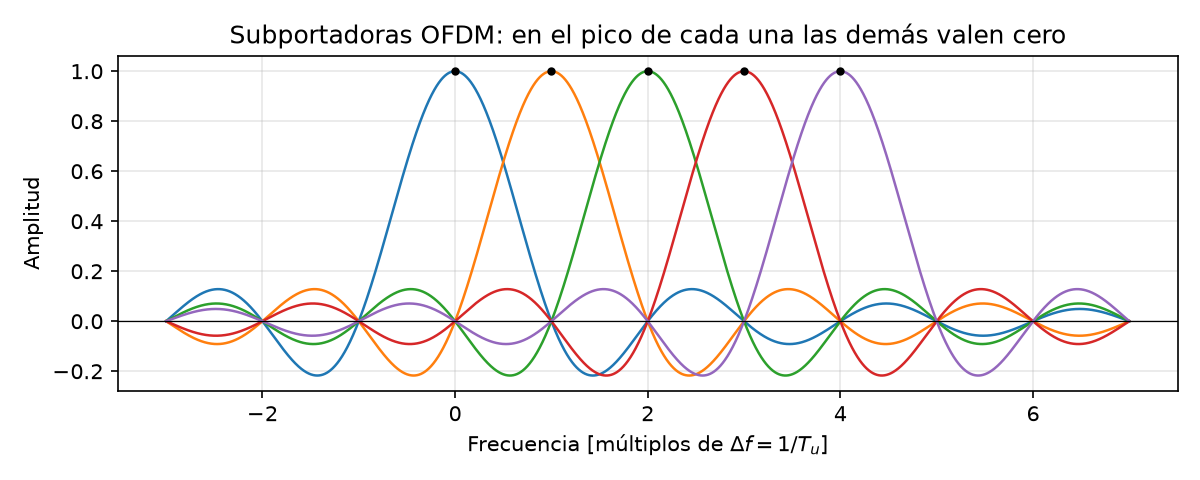
\includegraphics[width=\textwidth]{teoria/ofdm_subportadoras.png}
    \end{column}
  \end{columns}
  \note{\textbf{Agustín Mendes Rosa:} ISDB-Tb es la norma de la televisión digital abierta, que Argentina adoptó en 2009: toma la capa física japonesa y le agrega compresión H.264, audio AAC y el middleware Ginga. Su base es OFDM: el flujo de datos se reparte en miles de subportadoras lentas, separadas exactamente la inversa de la duración del símbolo, de modo que en el centro de cada una las demás pasan por cero. Cada símbolo dura cientos de microsegundos y lleva antepuesto un intervalo de guarda, así que los ecos que llegan dentro de ese intervalo no producen interferencia entre símbolos. Hay tres modos: más subportadoras dan símbolos más largos, que toleran ecos mayores pero son más sensibles al Doppler.}
\end{frame}

\begin{frame}{Segmentos y servicios en un mismo canal}
  \centering
  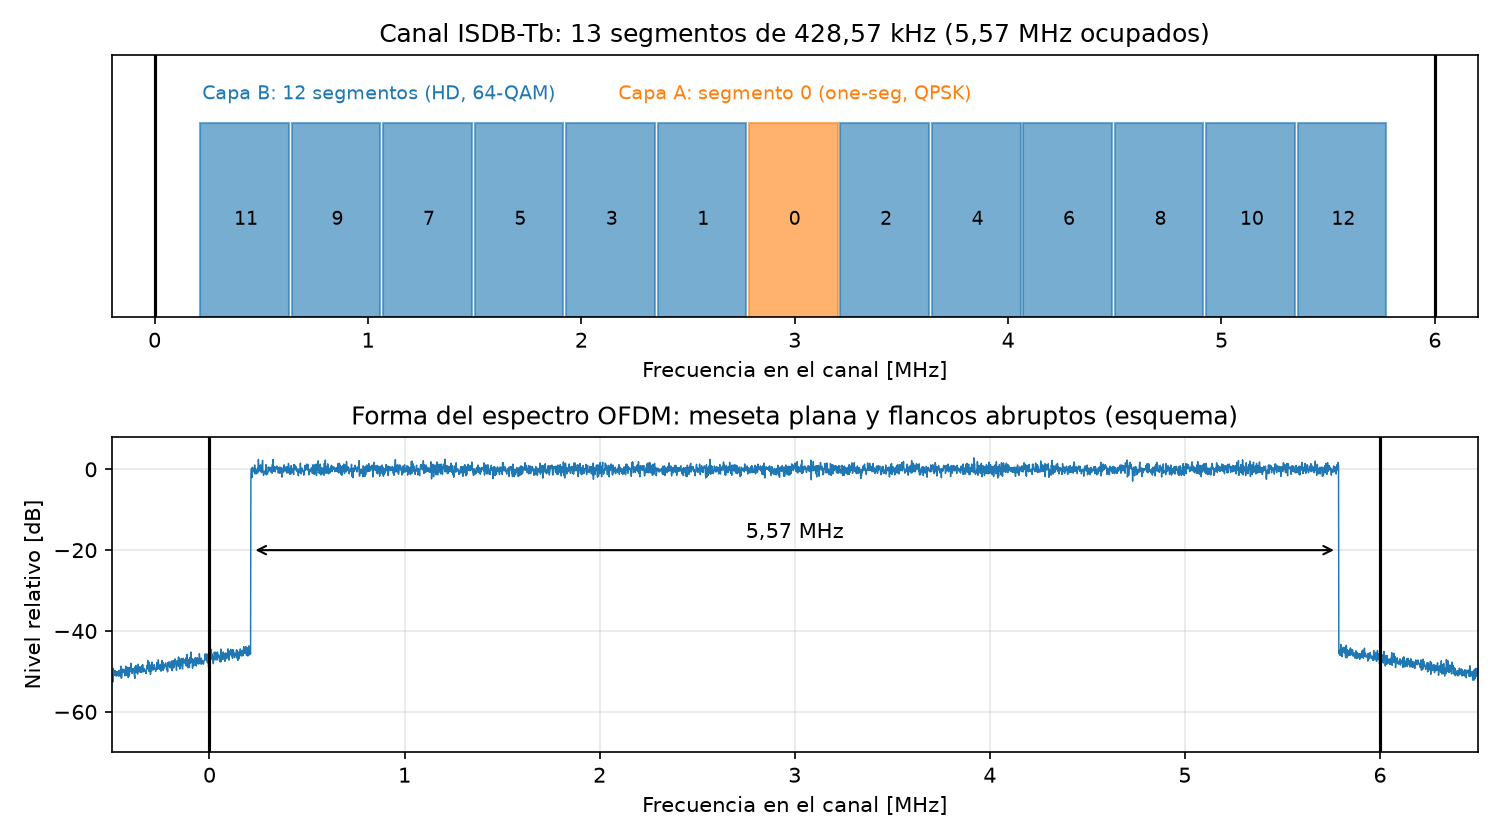
\includegraphics[width=0.66\textwidth]{teoria/isdbtb_segmentos.png}
  \vspace{0.1cm}

  \raggedright\small
  \begin{itemize}
    \item 13 segmentos de 428,57 kHz $\Rightarrow$ 5,57 MHz; portadoras TMCC con la configuración
    \item Hasta tres capas (A, B, C), cada una con su modulación, tasa de código y entrelazado
    \item Típico: capa A \textit{one-seg} (QPSK, $r = 2/3$) y capa B de 12 segmentos (64-QAM, $r = 3/4$)
  \end{itemize}
  \note{\textbf{Agustín Mendes Rosa:} El canal se divide en 13 segmentos de 428 kHz, que ocupan 5,57 MHz. Además de los datos, cada segmento lleva pilotos para estimar el canal y portadoras TMCC, que le informan al receptor la configuración, así que se configura solo. Los segmentos se agrupan en hasta tres capas jerárquicas, cada una con su propia modulación, tasa de código y entrelazado, y cada capa lleva su propio flujo de programas. Así se transmiten distintos servicios en un mismo canal. La configuración más usada tiene dos capas: el segmento central, el one-seg, para teléfonos y receptores portátiles, y los otros doce para alta definición.}
\end{frame}

\begin{frame}{Recepción fija y móvil; capacidad y robustez}
  \small
  \begin{columns}[T]
    \begin{column}{0.49\textwidth}
      \begin{block}{Recepción fija}
        Antena exterior directiva a $\approx 10$ m: buena SNR, canal estable $\Rightarrow$ 64-QAM con tasa alta.
      \end{block}
      \begin{block}{Recepción móvil y portátil}
        Antenas chicas, interiores o en vehículos: poca señal y multitrayecto $\Rightarrow$ QPSK, $r = 1/2$, entrelazado largo.
      \end{block}
    \end{column}
    \begin{column}{0.49\textwidth}
      \[ R_{seg} = \frac{96 \cdot \log_2 M \cdot r \cdot \frac{188}{204}}{T_u + T_g} \]
      \begin{itemize}
        \item 64-QAM, $r = 3/4$, guarda $1/8$: 1,40 Mbps por segmento; 16,8 Mbps en 12
        \item Canal completo: 3,65 a 23,2 Mbps
        \item Más capacidad $\Rightarrow$ menos robustez y SFN más chicas
      \end{itemize}
    \end{column}
  \end{columns}
  \note{\textbf{Agustín Mendes Rosa:} Para recepción fija, con una antena exterior directiva en el techo, el receptor tiene buena señal y un canal estable, y se pueden usar modulaciones densas como 64-QAM. En recepción móvil o portátil las antenas son chicas, la señal es menor y hay mucho multitrayecto, así que hacen falta modulaciones robustas como QPSK y entrelazado largo. La capacidad de cada segmento depende de la modulación, la tasa de código y el intervalo de guarda: con 64-QAM y tasa tres cuartos da 1,4 Mbps por segmento, 16,8 en una capa de doce, suficiente para un programa HD. El canal completo va de 3,65 a 23,2 Mbps, y cada aumento de capacidad se paga con robustez: más relación señal a ruido, menos corrección de errores o menos tolerancia a ecos.}
\end{frame}

% =====================================================
\section[ISDB-Tb cable]{ISDB-Tb sobre cable}
\orador{Vuelta 2}{Agustín Mendes Rosa}
\begin{frame}{ISDB-Tb sobre cable: propuesta, red y equipos}
  \small
  \begin{block}{En qué consiste}
    Canales ISDB-Tb, idénticos a los de la TDA, en la grilla de una red coaxial o HFC de $75\,\Omega$. Los televisores argentinos ya traen el sintonizador: \textbf{sin decodificador}. No hay norma específica: se aplica la terrestre.
  \end{block}
  \begin{columns}[T]
    \begin{column}{0.49\textwidth}
      \begin{block}{Cabecera}
        \scriptsize
        Receptores (satélite, fibra, IP) $\rightarrow$ codificadores H.264 $\rightarrow$ multiplexor-modulador ISDB-Tb (tablas PSI/SI, portadoras OFDM) $\rightarrow$ combinador RF
      \end{block}
    \end{column}
    \begin{column}{0.49\textwidth}
      \begin{block}{Red y recepción}
        \scriptsize
        La misma red de cable, cuidando niveles y planicidad. En el abonado: televisor con sintonizador ISDB-Tb, por coaxial.
      \end{block}
    \end{column}
  \end{columns}
  \note{\textbf{Agustín Mendes Rosa:} La propuesta de ISDB-Tb sobre cable es distribuir por la red de cable canales en la misma norma de la televisión digital abierta, en lugar de analógicos o DVB-C. Se usa sobre redes coaxiales o híbridas de 75 ohms. La ventaja es que los televisores vendidos en Argentina ya traen el sintonizador ISDB-Tb, así que reciben los canales sin decodificador. No encontramos una norma específica: se aplica la terrestre al cable. En la cabecera hacen falta receptores de las señales de origen, codificadores H.264, un multiplexor-modulador ISDB-Tb que arma los flujos con sus tablas y genera las portadoras OFDM, y un combinador. La red es la misma, cuidando los niveles, y en el abonado alcanza con el televisor.}
\end{frame}

\begin{frame}{Compatibilidad declarada y ejemplo comercial}
  \begin{columns}[T]
    \begin{column}{0.52\textwidth}
      \begin{block}{Según el fabricante (VideoSwitch)}
        \scriptsize
        \begin{itemize}
          \item Empresa argentina; modulador DMM-3100 ``ISDB-Tb Over Cable''
          \item Portadoras según ARIB STD-B31 y ABNT NBR 15601
          \item ``Permite la transmisión de televisión digital HD sin necesidad de agregar receptores externos al TV''
          \item Hasta 8 portadoras de 6 MHz, de 50 a 863 MHz; hasta 32 servicios por portadora
        \end{itemize}
        {\tiny Fuente: hoja de datos del DMM-3100. Prensa del sector: primera venta a Telecom.}
      \end{block}
    \end{column}
    \begin{column}{0.46\textwidth}
      \setbeamercolor{block title}{bg=grupo oeste,fg=white}
      \setbeamercolor{block body}{bg=grupo oeste!8}
      \begin{block}{Análisis propio}
        \scriptsize
        \begin{itemize}
          \item El TV debe sintonizar las frecuencias del operador, no sólo los canales 21 a 51
          \item Sin módulo de acceso condicional: programas sin cifrar
          \item Frente a DVB-C: 23,2 contra 38,5 Mbps por canal, pero compatible con el parque existente
        \end{itemize}
      \end{block}
    \end{column}
  \end{columns}
  \note{\textbf{Agustín Mendes Rosa:} La consigna pide separar lo que dice el fabricante. VideoSwitch, una empresa argentina, fabrica el DMM-3100, que según su hoja de datos genera portadoras según las normas ARIB y ABNT y permite transmitir HD sin receptores externos al televisor; según la prensa del sector, su primera venta fue a Telecom. Del análisis nuestro surgen dos condiciones: el televisor tiene que poder sintonizar las frecuencias que use el operador, y como los televisores no tienen acceso condicional, los programas van sin cifrar. Frente a DVB-C pierde capacidad, porque las herramientas de robustez de OFDM no hacen falta en el cable, pero para digitalizar sin entregar decodificadores, la compatibilidad pesa más. Cierra Luca.}
\end{frame}

% =====================================================
\section[Conclusiones]{Conclusiones}
\orador{Vuelta 2}{Luca Baccino}
\begin{frame}{Conclusiones: mediciones}
  \small
  \begin{itemize}
    \item \textbf{AM:} Cadena 3 y Radio Mitre, a 3 dB del ruido con una antena para VHF; ancho de banda y $f_{m,max}$ sólo teóricos. Con el generador, el peine de la cuadrada confirmó la serie de Fourier; con la senoidal, $m$ no pudo verificarse.
    \item \textbf{FM:} una docena de emisoras; $\approx 220$ kHz, entre Carson mono y estéreo; emisoras en canales adyacentes.
    \item \textbf{TV analógica:} canales 8, 10 y 12 (9 y 11 libres); video y audio separados 4,5 MHz, audio $\approx 10$ dB abajo; color en el canal 12.
    \item \textbf{TDA:} canal 27, meseta OFDM de $\approx 5{,}5$ MHz y $\approx -61$ dBm; sin prueba con televisor.
    \item \textbf{Niveles:} la conversión dBm--dBµV depende de la impedancia; los dBc no. Ejercicio: $m = 2$ \%.
  \end{itemize}
  \note{\textbf{Luca Baccino:} Para cerrar, los resultados de las mediciones. En AM identificamos las emisoras, pero con una antena para VHF quedaron casi en el ruido, así que el ancho de banda quedó en lo teórico; con el generador, la cuadrada mostró el peine que predice Fourier. En FM medimos unos 220 kHz, coherente con Carson, y encontramos emisoras en canales adyacentes. En televisión analógica ubicamos las portadoras de video, audio y color, y en la digital reconocimos el canal 27 por su meseta OFDM. Y en niveles, lo central es que para convertir entre potencia y tensión hay que conocer la impedancia.}
\end{frame}

\begin{frame}{Conclusiones: distribución y limitaciones}
  \small
  \begin{block}{Distribución por cable y fibra}
    DVB-C maximiza la capacidad con QAM; DOCSIS lleva datos e IP por la red HFC; el RF Overlay lleva la grilla de cable en 1550 nm sin decodificadores; ISDB-Tb usa OFDM en capas; sobre cable, aprovecha los televisores existentes.
  \end{block}
  \setbeamercolor{block title}{bg=grupo oeste,fg=white}
  \setbeamercolor{block body}{bg=grupo oeste!8}
  \begin{block}{Dificultades y limitaciones}
    \begin{itemize}
      \item Antena inadecuada para AM y piso de ruido del analizador ($\approx -100$ dBm)
      \item RBW comparable con el canal de AM y con las BL del generador
      \item Señales de programa variables; valores leídos sobre fotos de la pantalla
      \item Desadaptación 50/75 $\Omega$; no se dispuso de un receptor ISDB-Tb
    \end{itemize}
  \end{block}
  \note{\textbf{Luca Baccino:} En la investigación, cada tecnología resuelve un compromiso distinto: DVB-C maximiza la capacidad del cable, DOCSIS lo convierte en una red de datos, el RF Overlay lleva toda la grilla de cable por la fibra sin decodificadores, y ISDB-Tb permite combinar servicios fijos y móviles en un canal, y sobre cable aprovecha los televisores que ya hay. Las limitaciones principales fueron la antena, poco adecuada para AM, el piso de ruido del analizador, un RBW que no alcanzó para separar componentes cercanas, la variación de las señales de programa, que leímos los valores sobre fotos de la pantalla, y que no tuvimos un receptor para la televisión digital.}
\end{frame}

\begin{frame}[plain]
  \begin{tikzpicture}[remember picture, overlay]
    \fill[unc verde] (current page.north west) rectangle (current page.south east);
    \node[text=white, font=\Huge\bfseries] at (current page.center) {¡Gracias!};
    \node[text=white, font=\large] at ([yshift=-1.2cm]current page.center) {¿Preguntas?};
  \end{tikzpicture}
  \note{\textbf{Luca Baccino:} Muchas gracias. Si tienen preguntas, las respondemos entre todos.}
\end{frame}
